\documentclass[11pt]{article}

% Final (camera-ready) mode: non-anonymous, no review-mode line numbers.
% Per tasking/arxiv_paper.md Task 10: "final/non-anonymous mode."
\usepackage{acl}

% Standard package includes (from the ACL template, acl_latex.tex)
\usepackage{times}
\usepackage{latexsym}
\usepackage[T1]{fontenc}
\usepackage[utf8]{inputenc}
\usepackage{microtype}
% xurl lets the two long agency URLs in the bibliography break at any character
% instead of overflowing the column (two of the four pre-existing overfull boxes).
\usepackage{xurl}
\usepackage{inconsolata}
\usepackage{graphicx}
\usepackage{booktabs}
\usepackage{array}
\usepackage{tikz}
\usepackage{listings}
% Prompt listings. The prompts contain very long lines (single rules run to
% several hundred characters), so breaklines is essential; without it the
% appendix silently runs off the page edge rather than erroring.
\lstdefinestyle{promptstyle}{
  basicstyle=\scriptsize\ttfamily,
  breaklines=true,
  breakatwhitespace=false,
  breakindent=0pt,
  postbreak=\mbox{$\hookrightarrow$\space},
  columns=fullflexible,
  keepspaces=true,
  showstringspaces=false,
  frame=none,
  xleftmargin=0pt,
  aboveskip=4pt, belowskip=4pt,
  literate={—}{{---}}1 {–}{{--}}1 {≤}{{$\leq$}}1 {→}{{$\rightarrow$}}1
           {“}{{``}}1 {”}{{''}}1 {‘}{{`}}1 {’}{{'}}1 {…}{{\ldots}}1
           {≥}{{$\geq$}}1 {×}{{$\times$}}1 {½}{{$\frac{1}{2}$}}1
}

% ---------------------------------------------------------------------
% Float spacing. Two independent sources of whitespace, both from LaTeX
% defaults rather than from anything in this paper:
%   1. \textfloatsep / \floatsep / \dbltextfloatsep are generous, so every
%      float carries ~20pt of separation above and below it.
%   2. On a FLOAT-ONLY page (this paper produces two: the architecture
%      figure with the two headline tables, and the appendix corpus pair)
%      the defaults \@fptop/\@fpsep/\@fpbot each carry `fil` glue, which
%      distributes the floats over the full page height instead of setting
%      them from the top. That is what made those pages read as mostly gap.
% Raising \topfraction and \floatpagefraction additionally lets a float sit
% on a text page rather than being deferred onto a float-only page at all.
% None of this touches margins, type size or the ACL page geometry.
% ---------------------------------------------------------------------
\setlength{\textfloatsep}{12pt plus 2pt minus 2pt}
\setlength{\floatsep}{10pt plus 2pt minus 2pt}
\setlength{\intextsep}{10pt plus 2pt minus 2pt}
\setlength{\dblfloatsep}{10pt plus 2pt minus 2pt}
\setlength{\dbltextfloatsep}{12pt plus 2pt minus 2pt}
\setlength{\abovecaptionskip}{6pt}
\setlength{\belowcaptionskip}{0pt}
\makeatletter
\setlength{\@fptop}{0pt}
\setlength{\@fpsep}{14pt plus 4pt}
\setlength{\@fpbot}{0pt plus 1fil}
\setlength{\@dblfptop}{0pt}
\setlength{\@dblfpsep}{14pt plus 4pt}
\setlength{\@dblfpbot}{0pt plus 1fil}
\makeatother
\renewcommand{\topfraction}{0.9}
\renewcommand{\dbltopfraction}{0.9}
\renewcommand{\bottomfraction}{0.7}
\renewcommand{\textfraction}{0.1}
\renewcommand{\floatpagefraction}{0.8}
\renewcommand{\dblfloatpagefraction}{0.8}

\title{Classify by Position, Not by Label: LLM-Driven Extraction of Hierarchical Structure from Fragmented US Early Learning Standards}

\author{
  Emily Cheyne \\
  Founder, EdTech Co. \\
  \texttt{emily@edtechco.org}
}

\begin{document}
\maketitle

\begin{abstract}
Every US state publishes early learning standards, the developmental
expectations for children from birth to kindergarten, and each designs its
own document, so software cannot read this public policy. The obstacle is not
text recovery but hierarchy recovery: a standard is meaningful only through its
ancestry, and the surface cues that reveal ancestry are exactly what varies.
Arizona writes \texttt{Strand 1:}, Kentucky writes \texttt{Benchmark 1.1},
Nevada's code namespace skips a level, and Colorado has no sub-strand tier at
all.

I present an LLM-driven method that classifies each element by its
\emph{nesting position} rather than its label vocabulary. A first pass infers a
per-document depth map and a second classifies every element against it; a
decoupled parser resolves the result into one canonical schema with
deterministic identifiers, and a serverless batching
architecture applies it to whole documents. There is no per-state code path,
though the prompts carry worked examples from the corpus
(\S\ref{sec:method-discipline}).

On an annotated subset of four development states and two held out entirely,
detector recall is 1.000 at every hierarchy level in all six, and a manual audit
of all 297 in-scope detections finds one hallucinated element. Ablating the
depth map leaves domain and indicator recall untouched while strand falls to
0.920 and sub-strand to 0.833, exactly the levels whose identity is positional,
and a rule-based extractor matches the method at the top division but collapses
beneath it. Repeated runs show the pipeline is not deterministic, with
instability concentrated in three known places, and one of my own earlier
results failed to reproduce; I report it as a non-reproduction. That reporting
discipline is offered as a contribution: every table names its corpus tier,
every unmatched detection is audited by hand, and every number is regenerated
from a recorded artifact.
\end{abstract}

% Section order reconstructed from the original outline (paper/OUTLINE_NOTES.md)
% and shortened 2026-09-07 (REVIEW_assessment.md §2): the standalone pipeline
% overview is folded into \S\ref{sec:method}, and the system architecture is
% Appendix~\ref{sec:appendix-architecture}.

\section{Introduction}
\label{sec:introduction}

Every US state publishes early learning standards: the developmental
expectations that shape curriculum, assessment, and teacher preparation for
children from birth through kindergarten entry. More than fifty jurisdictions
issue them independently~\citep{ncecqa_elgs,ecs2024governance}, and each designs its
own document. The result is a body of policy that is public, consequential, and
almost entirely unavailable to software. Unlike K--12 academic standards, which
have machine-readable distribution
formats~\citep{sutton2008achievement,1edtech2017case}, early learning standards
exist as PDFs --- multi-column tables, age-banded grids, and prose narratives
whose typography is shared by no two states.

The obstacle is not optical character recognition. It is that a standards
document is a \emph{tree} rendered as a page. A single indicator is meaningful
only through its ancestry: which domain, which strand, which sub-strand it sits
under, and at what age band. Recovering that tree requires deciding, for every
line, how deeply it is nested --- and the surface cues that would answer the
question are exactly what varies between states. Arizona writes
\texttt{Strand 1: Language and Literacy}; Kentucky writes
\texttt{Benchmark 1.1}; Nevada prints a code namespace that skips a level
entirely; Colorado publishes no sub-strand tier at all. A rule tuned to one
document's vocabulary is, by construction, a rule that fails on the next.

My central claim is that a language model can recover this structure by
classifying each element's \textbf{nesting position} rather than its
document-specific label, and that doing so is what generalizes. Concretely, I
first infer a per-document \emph{depth map} --- how many nesting levels this
particular document uses, and what each looks like --- and then classify every
element against that map as an authority, rather than against a fixed
vocabulary of level names. The label \texttt{Benchmark 1.1} then does not have
to be recognized as a sub-strand; it has to be recognized as sitting one level
below whatever \texttt{Language and Early Literacy Standard 1} is.

This framing also determines how the system is built. I hold a deliberate
design discipline that structural decisions belong in the prompt as general
document principles, not in Python as per-document branches. That discipline
was adopted after an earlier rule-driven revision scored well on the states it
had been developed against and failed to transfer; the migration that removed
those rules is described in \S\ref{sec:method-llm-first}. Deterministic code is
retained only where it reads the \emph{shape} of an output --- dot-segment
structure, whitespace, string containment --- and never any document's words.

The absence of a labeled corpus is what rules out the obvious supervised
alternative. There is no annotated dataset of hierarchically-parsed early
learning standards at any scale, so a fine-tuned model would first require one
to be built, and the dominant cost of that path is annotation rather than
compute. My own goldens took expert effort to produce and cover six states;
they are an evaluation instrument, not a training set. An in-context approach
that needs no labeled data is therefore not merely cheaper here, it is the only
approach available without first solving a different problem
(cf.~\citealp{liu2022fewshot} for the counterargument where labels do exist).

\paragraph{Contributions.}
\begin{enumerate}
  \item A two-stage detection method built on per-document depth-map inference
    and classify-by-nesting-position prompting, with no per-state code path
    (\S\ref{sec:method-detection}; what the prompts do carry is itemized in
    \S\ref{sec:method-discipline}).
  \item A parsing stage that resolves detected elements into a single canonical
    schema across documents that do not agree on level count or code namespace,
    producing deterministic, collision-free identifiers
    (\S\ref{sec:method-parsing}).
  \item A serverless architecture that batches detection and parsing through a
    prepare--map--merge pattern so the method applies to whole standards
    documents rather than excerpts (\S\ref{sec:method-deployment},
    Appendix~\ref{sec:appendix-architecture}).
  \item An evaluation over four development states and two held-out states.
    Detector recall is 1.000 at every hierarchy level in all six states, and a
    manual audit of all 297 in-scope detections finds a single hallucinated
    element (verified precision 0.997). An ablation shows the depth-map pass is
    what carries the intermediate levels: removing it leaves domain and
    indicator recall untouched while strand falls to 0.920 and sub-strand to
    0.833 (\S\ref{sec:experiments-ablation}).
  \item A reporting discipline that the rest of the evaluation is built to
    satisfy, and which I offer as a contribution rather than as a caveat: every
    table is labelled with the corpus tier it was computed at; every unmatched
    detection is audited by hand and signed rather than assumed to be a false
    positive; every number is regenerated from a recorded artifact by a named
    script; a validation guard is shown catching a live defect rather than
    asserted to work; and a previously recorded result of my own that failed to
    reproduce is reported as a non-reproduction instead of quietly replaced
    (\S\ref{sec:experiments-stability}, \S\ref{sec:discussion-limitations}).
\end{enumerate}

\paragraph{Scope of the reported numbers.} Every headline quality measurement
in this paper is computed at the \emph{subset} corpus tier: hand-trimmed
excerpts of one to two domains per state, 70 pages in total, fully annotated.
This is favorable preprocessing and I state it plainly rather than leaving it to
be inferred; \S\ref{sec:corpus} gives the tiers and retained page ranges, and
\S\ref{sec:discussion-limitations} discusses what does and does not transfer to
whole documents. Cost, scale and one quality measurement are reported at the
\emph{trimmed} tier instead---a document's standards content in full, with front
matter, expository essays and appendices removed. The tiers are never mixed
within a table, and each table names its own
(\S\ref{sec:experiments-scale}, \S\ref{sec:experiments-scale-quality}).

% related_work.tex — Task 9 deliverable (drafted 2026-08-17); condensed and
% re-argued 2026-09-05. The 2026-08-17 draft enumerated systems roughly one per
% sentence and ran ~940 words. Each subsection now carries a single claim and
% groups its citations under it, at ~735 words (-22%). Citation COVERAGE is
% unchanged — every key cited by the earlier draft is still cited here, and
% nothing else in the paper cites a key that this section dropped.
% Citations use natbib (\citep/\citet) against ../references.bib.
% Guardrails observed: no unmeasured Medium numbers; no confidence-gate claim
% (verification is blanket, confidence gates nothing); no invented fine-tuning
% cost comparison — the in-context argument is made on no-labeled-corpus grounds.
% One factual softening vs. the 2026-08-17 draft: aggarwal2025fiscal is credited
% with validating against the documents' "own internal consistency", not
% specifically their "arithmetic structure", which REVIEW_references.md
% (2026-09-04) could not confirm from the abstract.

\section{Related Work}
\label{sec:related}

\subsection{Hierarchy recovery from documents}

Recovering logical structure from formatted documents has a long lineage ---
scholarly-PDF pipelines~\citep{lopez2009grobid}, page-object
datasets~\citep{zhong2019publaynet}, layout-aware
encoders~\citep{xu2020layoutlm,huang2022layoutlmv3}, OCR-free
vision--encoder--decoder models~\citep{kim2022donut,blecher2023nougat} --- but
its targets are flat: classification, key--value extraction and markup
transcription rather than a tree. Work that does reconstruct the tree parses it
from renderings~\citep{rausch2021docparser}, decomposes it into page-object
detection, reading order and tree
construction~\citep{ma2023hrdoc,wang2024detect}, recasts those subtasks as
relation prediction~\citep{wang2025unihdsa}, extends them to multi-domain
corpora~\citep{xing2024dochienet}, or reads table-of-contents metadata from
deeply nested legal books~\citep{wehnert2025hips}.

These systems differ in architecture but share a premise, and it is the
premise rather than any individual design that my setting violates: hierarchy
can be \emph{learned}, because supervision exists --- line labels, bounding
boxes, TOC metadata, pretraining on labeled pages --- over a genre whose
typography is internally consistent. Early learning standards offer neither.
With every jurisdiction designing its own document~\citep{ncecqa_elgs}, there
is no shared typography to learn and no annotated corpus, at any scale, to
learn it from.
What the documents do share is not appearance but nesting: whatever a level is
called, it sits at a fixed depth relative to its neighbors. My depth-map pass
is functionally the table-of-contents subtask of \citet{wang2024detect}, but
inferred zero-shot from content rather than predicted by a trained component,
then treated as the authority against which every element is classified. The
closest zero-shot neighbor, DocsRay~\citep{jeong2025docsray}, likewise prompts
for a pseudo table of contents with no training, but targets a segmentation
guiding retrieval for question answering rather than a typed hierarchy carrying
codes and ancestry, and is not graded against structural annotations.

\subsection{In-context extraction without a labeled corpus}

Prompting alone carries many tasks~\citep{brown2020language}, including
multi-step reasoning~\citep{wei2022chain}, and generative extraction is now
competitive across classic IE
tasks~\citep{wadhwa2023revisiting,xu2024large}, notably where labeled corpora
are scarce~\citep{agrawal2022large}. GoLLIE~\citep{sainz2024gollie} is the
closest methodological analogue: fine-tuning a model to follow annotation
\emph{guidelines} makes it generalize to unseen schemas. My prompts
operationalize that insight without fine-tuning, stating document-agnostic
structural principles (e.g., a structural label and its identifier constitute
the code; the text after the colon is the title) that a frozen model applies to
unseen states. This is the available move rather than merely the cheap one: no
annotated corpus of parsed early learning standards exists, so the supervised
alternative's dominant cost would be annotation, not compute
\citep[cf.][where labels do exist]{liu2022fewshot}.

Three system choices follow: schema-validated JSON with deterministic repair
rather than constrained decoding~\citep{willard2023efficient}, which keeps the
method API-agnostic; domain-scoped chunking
(\S\ref{sec:system-architecture}) rather than whole-document prompting, given
positional degradation in long contexts~\citep{liu2024lost}; and reported
run-to-run stability (\S\ref{sec:experiments-stability}) rather than a single
run, given sampling variance at fixed prompts~\citep{wang2023selfconsistency}.
Hallucination, the residual risk of generative extraction~\citep{ji2023survey},
I quantify by auditing every unmatched detection by hand. The nearest applied
system~\citep{aggarwal2025fiscal} converts government fiscal PDFs into a
research database with a multi-stage LLM pipeline validated against the
documents' own internal consistency; standards documents afford the analogous
check on their \emph{hierarchical} consistency --- codes as namespace paths,
parent--child prefix relations.

The absence of labels also decides where human effort goes: to verification
rather than annotation. Every extracted record is human-reviewed at all four
hierarchy levels --- the model drafts, humans supply the correctness guarantees
it cannot --- following the machine-teaching paradigm of experts controlling
the process rather than labeling
data~\citep{mosqueirarey2023human,monarch2021human}. It differs from active
learning~\citep{settles2009active} and from work allocating annotation between
models and humans~\citep{gilardi2023chatgpt,li2023coannotating,tan2024large} in
that verification is blanket, not selective: nothing decides \emph{which}
records a human sees, and the detector's confidence scores are recorded but
gate nothing.

\subsection{Machine-readable education standards}

Two decades of work on standards as data share one assumption. The Achievement
Standards Network modeled US K--12 standards in
RDF~\citep{sutton2008achievement} and the CASE specification defines an
exchange format for competency frameworks~\citep{1edtech2017case}, but ASN was
populated by manual modeling and CASE is a format, not an extractor.
Downstream, alignment between standards, assessments and instruction is
measured by trained human
panels~\citep{porter2002measuring,polikoff2011howwell}, while NLP from the ASN
era onward assigns learning resources~\citep{devaul2011computer} and, more
recently, assessment items~\citep{xu2025automated} \emph{to} standards already
normalized. For early childhood the assumption fails outright: no national
framework spans the age band --- the federal ELOF covers Head Start programs
only~\citep{ohs2015elof} --- and each state publishes its own guidelines as an
independently designed PDF~\citep{ncecqa_elgs,ecs2024governance}. The extraction
step this paper automates is not a competitor to that literature but its
missing input.

\section{Corpus}
\label{sec:corpus}

The corpus is the early learning standards documents of six US states: four
used for development (Arizona, California, Colorado, Texas) and two held out
entirely (Nevada, Kentucky). Table~\ref{tab:dataset-stats} summarizes what the
annotated portion of each contains; Appendix~\ref{sec:appendix-corpus} names
every source document and lists the pages retained at each tier.

Each document exists at up to three tiers, and the two reductions are not the
same kind of reduction. The \emph{full} tier is the published PDF as issued.
The \emph{trimmed} tier removes non-standards matter (front matter,
introductions, guiding-principles essays, appendices, acknowledgements) and
\textbf{retains every standard}; it reduces page count, and therefore cost, but
not coverage, and it is the tier the scale measurements of
\S\ref{sec:experiments-scale} and \S\ref{sec:experiments-scale-quality} run on.
Kentucky's 52 trimmed pages are all of Kentucky's standards. The \emph{subset}
tier is a genuine reduction in coverage: one to two domains per state, 8--15
pages each and 70 in total, chosen to be cheap to iterate on and to annotate
exhaustively. \textbf{Every headline quality number in this paper is computed
at this tier}; the one quality measurement at the trimmed tier
(\S\ref{sec:experiments-scale-quality}) is kept in its own table. Both cuts
were made by hand, which is favorable preprocessing; Table~\ref{tab:corpus-pages}
lists the retained pages so that either tier can be reconstructed from the
issuing agency's copy. It gives two numberings, because they are not the same
number: a page's index in the PDF file, and the page number printed on the
page, which differ by each document's unnumbered front matter. Kentucky's PDF
page 52 is printed page 39, and its subset also contains PDF page 65, whose
printed number is 52, so ``page 52'' is ambiguous on that document alone.
Printed numbers are recovered automatically and are reported only for the two
documents where that recovery is reliable across the whole tier.

Two sources need naming precisely. California's document is the state's
Preschool/Transitional Kindergarten Learning Foundations ``at a glance''
publication (68 pages), which was cut directly to its 13-page subset with no
trimmed tier. Colorado's is the 41-page Ages~3--5 volume of the state's
birth-to-eight guidelines; its trimmed tier is the whole document, so nothing
was cut from it, and its out-of-scope content is other age bands rather than
standards removed by trimming. The held-out canary is Nevada's 2023
pre-kindergarten standards, a multi-domain document; a separate Nevada
publication from 2025 covering only the social-emotional domain was collected
but is too narrow to support a generalization claim and is excluded from every
measurement (Table~\ref{tab:corpus-appendix}).

Two properties of Table~\ref{tab:dataset-stats} are results rather than
document facts. Its age-band column counts the distinct bands a state uses,
not coverage: every one of the 262 standards carries an age band. And
identifier collisions are zero in every state, which matters because the
identifier is the key under which a standard is stored (\S\ref{sec:schema}).

% AUTO-GENERATED by paper/analysis/generate_tables.py -- do not hand-edit.
% Source: paper/results/task8_20260904/dataset_stats.json
% Regenerate with: python paper/analysis/generate_tables.py
% Corpus tier (guardrail 1): every row is the _only_subset tier, never full-document.
\begin{table*}
  \centering
  \begin{tabular}{llrrrrrrrr}
    \hline
    \textbf{State} & \textbf{Role} & \textbf{Subset pp} & \textbf{Full pp} & \textbf{Dom.} & \textbf{Str.} & \textbf{Sub.} & \textbf{Standards} & \textbf{Age bands} & \textbf{ID coll.} \\
    \hline
    AZ & golden & 15 & 217 & 2 & 4 & 9 & 45 & 1 & 0 \\
    CA & golden & 13 & 68 & 3 & 7 & 18 & 94 & 3 & 0 \\
    CO & golden & 10 & 41$^{\dagger}$ & 3 & 10 & 0 & 48 & 1 & 0 \\
    TX & golden & 9 & 87 & 2 & 4 & 2 & 25 & 2 & 0 \\
    NV & held-out & 15 & 98 & 3 & 7 & 7 & 24 & 1 & 0 \\
    KY & held-out & 8 & 120 & 3 & 5 & 10 & 26 & 1 & 0 \\
    \hline
    \textbf{Total} & & 70 & & 16 & 37 & 46 & 262 & 6 & \textbf{0} \\
    \hline
  \end{tabular}
  \caption{Corpus descriptive statistics. Domain, strand and sub-strand columns count \emph{distinct} nodes in at least one standard's ancestor chain, so they are smaller than the detector's element counts in Table~\ref{tab:detector-headline}. \textbf{Age bands} is the state's distinct bands; its total is the union across states, not a column sum. CO's subsets derive from the 41pp ages-3--5 document ($\dagger$). All quality numbers in this paper are measured on the \emph{\_only\_subset} tier shown here (\S\ref{sec:corpus}). Source: \texttt{task8\_20260904}.}
  \label{tab:dataset-stats}
\end{table*}


% schema.tex — Task 10 stub. Reconstructed section (see ../OUTLINE_NOTES.md).
% Draft at Task 12. Outline:
%   - The canonical target hierarchy: domain -> strand -> sub_strand (optional)
%     -> indicator, each level with code/name/description/age_band.
%   - standard_id format: {country}-{state}-{year}-{indicator_code}, fully
%     qualified, deterministic, no separate domain_code component
%     (src/els_pipeline/parser.py generate_standard_id; models.py is the
%     Python source of truth, packages/shared/src/types.ts mirrors it).
%   - Why a single canonical schema across 50+ independently-formatted state
%     documents is itself a nontrivial contribution — most states do not
%     share a level count (CO has no sub_strand) or a code namespace shape.
%   - Point forward to Appendix~\ref{sec:appendix-schema} for the full
%     schema and Appendix~\ref{sec:appendix-goldens} for annotated examples.

\section{Canonical Schema}
\label{sec:schema}

\section{Method}
\label{sec:method}

The system is a six-stage pipeline. \textbf{Ingestion} registers a source PDF
and its provenance. \textbf{Extraction} recovers text blocks with their page
numbers and page coordinates, using a hybrid of OCR and the PDF's own text
layer, since either alone is unreliable on the multi-column and tabular layouts
these documents favor. \textbf{Detection} is where structure is recovered,
emitting a flat list of typed elements, each carrying a level, a code, a title,
an optional description, an age band, and the source text it was read from.
\textbf{Parsing} resolves that flat list into the canonical schema of
\S\ref{sec:schema}, attaching each indicator to its full ancestry and composing
its identifier. \textbf{Validation} checks each record against the schema and
against structural invariants on the identifier, and \textbf{persistence}
writes the surviving records to a relational store. The two stages that recover
structure are the subject of this section.

\subsection{Two-Stage Design Rationale}
\label{sec:method-two-stage}

Recovering a standards hierarchy involves two decisions that are easy to
conflate and better kept apart: \emph{what is on the page}, and \emph{what it
is a child of}. The first is local (a heading, a numbered item, a paragraph of
prose) and can be judged from the text in front of the reader. The second is
global: an element's parent may be several pages back, may be printed only once
at the top of a section that runs for multiple pages, or may not be printed at
all and must be recovered from the codes of its own descendants. Detection is
accordingly forbidden from reconstructing an absent parent out of the position
identifiers inside a child's code, and emits the children alone
(Appendix~\ref{rule:emit-what-you-see}); recovering that parent is parsing's
work, not detection's.

I therefore split the work. \textbf{Detection} reads the document in
overlapping chunks and emits a flat list of typed elements, each labeled with
its hierarchy level but not linked to a parent. \textbf{Parsing} takes that flat
list, groups it by domain, and resolves each indicator's full ancestry and
identifier. The split buys three things. It lets each stage see the context it
actually needs, so parsing reasons over an entire domain's elements at once
rather than over one chunk's worth of text. It lets the two stages be graded
independently against separately annotated goldens, which is what makes a
detection failure distinguishable from a resolution failure. And it lets the two
stages run on different models, since they are not equally hard
(\S\ref{sec:method-model-assignment}).

\subsection{Detection}
\label{sec:method-detection}

Detection is two passes over the extracted text blocks.

\paragraph{Pass 1: depth-map inference.} Before any element is classified, a
single cheap model call infers the document's \emph{depth map}: how many nesting
levels this document uses, and what an element at each level looks like in it.
This is the paper's central move. Rather than asking the model to recognize
``strand'' or ``benchmark'' as level names, vocabulary that no two states
share, I ask it once, per document, to characterize that document's own
nesting scheme, and then treat the answer as authority for every subsequent
classification. Appendix~\ref{sec:prompt-depthmap} gives that prompt in full;
it is short, and it is the only one reproduced whole.

The pass runs on a sample of blocks rather than the whole document, under a
6{,}000-token budget, and how that sample is drawn turns out to matter a great
deal. Because every element's level is assigned against the map, \emph{a level
missing from the sample is a level missing from the entire run}: if the sample
contains no evidence that a document nests four deep, the map reports three, and
every element below the missing level is shifted up one.

The obvious sampler, keeping every $n$th block, is the wrong one here. It
keeps each line with the same probability $1/n$ however much structural evidence
that line carries, and in a standards document evidence and frequency run
opposite to one another: a section heading appears once per section, while the
body prose beneath it is repeated on every page. Uniform sampling therefore
drops precisely the headings that establish the top of the hierarchy and keeps
the prose, which establishes nothing, on volume alone.

I stratify by layout instead. Extraction already records each block's normalized
left edge, and that edge is already part of what the model is shown; since
indentation tracks nesting, a rare horizontal position \emph{is} a rare depth.
Blocks are therefore bucketed by left edge, and each bucket is guaranteed a
floor of twelve blocks spread across the document. Buckets are filled
rarest-first, so when the budget binds, what it truncates is the bulk of the
document rather than the structurally distinctive levels. The guarantee is cheap
for the same reason it is needed: those levels are rare, and in Kentucky's
complete standards document the heading buckets together hold only a small
fraction of all blocks.\footnote{An observation from the project's engineering
notes rather than a recorded experiment.} Blocks whose page geometry is unusable
have no left edge to group on, and fall back to a coarse text-shape key reading
word count and final character only. Either way the rule reads layout position
and counts, never any document's words.

\paragraph{Pass 2: classification against the map.} The document is then chunked
into roughly 2{,}000-token windows with 500 tokens of overlap, and each chunk is
classified with the depth map supplied as context. The overlap exists because
elements straddle chunk boundaries; because chunks overlap, a long description
split across a boundary can be reconstructed by splicing the shared span, which
recovers passages that neither chunk holds whole.

The prompt states general document-structure principles rather than per-state
rules. Its central instruction is positional: classify an element by where it
sits in the depth map, not by the word its label happens to use
(Appendix~\ref{rule:positional}). Supporting
rules are stated at the same level of generality: a heading of the form
\texttt{<Label> <id>: <Title>} has the label-and-id as its code and the text
after the colon as its title, for \emph{any} structural label word rather than a
fixed list; a code, when the document prints one, is authoritative and may
appear inline, in a caption beside the heading, or as the shared leading prefix
of its descendants' codes; and when the document prints none, a code is
derived from the title by a stated abbreviation procedure capped at five
characters. All three are one rule, reproduced at
Appendix~\ref{rule:code-resolution}.

\paragraph{Where determinism is enforced in code.} The last of those rules,
deriving a code from the element's title when the document prints none, is
different in kind from the others. The rest ask the model for a judgement about
a document; this one asks it to execute a deterministic string algorithm, and a
sampling model executes such an algorithm inconsistently. In an engineering
measurement on Kentucky (three runs at temperature zero against one frozen
extraction, recorded in the project's design notes rather than as a paper
artifact) roughly a quarter of the elements received a different code on at
least one run, while level, source page, and age band never varied. Because the
code becomes part of a database primary key, a rate near zero is not good
enough. The abbreviation is therefore also executed in Python, but only where
the document supplied no code of its own, decided by two independent guards: a
\emph{shape} guard, since the abbreviation branch emits uppercase letters and
nothing else, so a code carrying a digit, separator, or lowercase letter is
positional and is never touched; and a \emph{grounding} guard, since a code read
off the page appears in the element's own source text while an invented
abbreviation does not. Both are required: a model that transcribes a lettered
item without its list prefix defeats grounding alone.

This is a pairing, not a substitution. The rule stays in the prompt verbatim;
the code makes its floor zero. The same pattern recurs throughout the system,
and \S\ref{sec:method-llm-first} states the discipline that governs it.

\subsection{Parsing}
\label{sec:method-parsing}

Parsing consumes the flat element list, batched by domain so that an entire
domain's elements are resolved together, and produces normalized standards.

The substantive work is composing each indicator's fully-qualified code from its
chain of ancestors, and the difficulty is that printed code namespaces are not
uniform. Three shapes recur. A namespace may \emph{skip} a level, as Nevada's
does: its sub-strand code does not extend its strand code, and requiring it to
would corrupt every one of the 24 annotated Nevada standards, all of which break
the chain at exactly that level. A sub-level identifier may be
\emph{dotted}, restating its parent's position inside its own id, as Kentucky's
\texttt{Benchmark 1.1} does, whose leading \texttt{1} \emph{is} Standard~1; so
composing it onto the full parent code counts that parent twice. And a heading
may print a label-and-id form that must be converted into the domain-qualified
form before it can be composed at all (Appendix~\ref{rule:label-identifier}).

Each is handled by a rule keyed on structure rather than vocabulary. Peeling an
ancestor's code from a descendant's stops where the namespace stops: if a level's
anchored code would equal the code of the level directly below it, the peel has
run past the end of the namespace and that level keeps its own heading's
identifier (Appendix~\ref{rule:namespace-skip}). A code that already carries its
own qualification is used as it stands and is never qualified a second time, at
any level (Appendix~\ref{rule:already-qualified}). A dotted child whose added segment repeats its parent's last segment
is collapsed, but only when the added tail is itself dotted, since a single added
segment is an ordinary child index. A repair that cannot demonstrably improve the
row's own ancestry is not made, and a repair that would introduce whitespace into
an identifier declines rather than trading one malformation for another. None of
these rules contains a list of label words; whitespace and dot structure are the
only signals they read.

Uniqueness is enforced after the merge rather than during it, because a collision
can span batches. Colliding standards are re-qualified using their own ancestors'
segments, and \emph{every} member of a colliding set is rewritten, including the
first one seen, so the result does not depend on the order in which chunks
arrived. Where two standards share every ancestor and remain indistinguishable, a
numeric suffix is assigned in document order. That is reproducible, but it
carries no information, which is why it is a last resort and is logged as one.

Finally, a validation stage rejects any record whose codes are structurally
impossible before it reaches the database: no code may contain whitespace, the
indicator's code must extend its nearest present ancestor's, and the identifier
must end with the indicator code. The middle condition is deliberately scoped to
the leaf, because, as Nevada shows, an intermediate level may legitimately
break the chain.

\subsection{Model Assignment}
\label{sec:method-model-assignment}

The three model calls in the pipeline are not equally difficult, and I assign
the cheapest model that suffices for each. The depth-map pass produces a short
structural summary from a sampled fraction of the document and runs on Claude
Haiku 4.5. Detection is the hard classification problem and runs on Claude Opus
4.6. Parsing operates on already-typed elements with the ancestry constraints
supplied explicitly, and runs on Claude Sonnet 4.6. Since detection is the only
stage invoked once per chunk of the whole document, this assignment also
concentrates spend where the difficulty is. I state the principle here as a
design commitment; \S\ref{sec:experiments-results} reports what the assignment
costs, and a model-tier ablation is identified as future work rather than
claimed as evidence.

\subsection{Confidence and Human Verification}
\label{sec:method-confidence}

Every detected element carries a confidence score, and \textbf{nothing in the
pipeline thresholds it}. There is no review gate, no minimum score, and no
field marking an element as requiring attention; all elements flow through
detection, parsing, validation, and persistence regardless of score. The prompt
does ask for a band, and Appendix~\ref{rule:confidence-bands} reproduces what it
asks for; nothing downstream reads the answer. I am
explicit about this because it is easy to assume otherwise, and because my own
measurement of the score's distribution argues against building such a gate: the
scores occupy five distinct values in $[0.90, 0.97]$, the band the prompt
describes as indicating uncertainty is used zero times, and the score varies
more by document than by whether an element is correct
(\S\ref{sec:experiments-confidence}).

Human verification is a separate mechanism. The schema carries per-element
verification state at all four levels, and an editorial interface lets a
reviewer confirm or correct each element against the source PDF. It is a
workflow over the stored corpus, not a filter applied during extraction, and it
is blanket rather than score-triggered.

Whether every standard must be verified before the corpus is useful is
therefore a cost-and-trust decision rather than a precondition. The durable win
is that fifty independently-formatted documents become one queryable corpus,
and that value is available before every leaf has been signed off, provided the
verification state travels with the data so a consumer can decide what it
requires: uses carrying regulatory or assessment weight will reasonably demand
verified records, exploratory ones reasonably will not.

\subsection{Deployment}
\label{sec:method-deployment}

The method is deployed as a serverless pipeline whose stages communicate by
writing JSON to S3 rather than by passing payloads directly, so each stage's
input and output can be inspected in isolation when a run is debugged.
Detection and parsing are batched through a prepare $\rightarrow$ \texttt{Map}
$\rightarrow$ merge pattern with at most three concurrent workers, so that a
long document does not exhaust a function timeout; detection batches by
text-block chunk and parsing by domain, which keeps related elements in the
same call. Appendix~\ref{sec:appendix-architecture} gives the deployed
architecture and the interface through which the extracted corpus is reviewed.

\textbf{The evaluation suites exercise the direct path rather than this batched
one, and the two are known to diverge}
(\S\ref{sec:discussion-limitations}). Every subset-tier quality number in this
paper is therefore a measurement of the direct path;
\S\ref{sec:experiments-scale} and \S\ref{sec:experiments-scale-quality} are the
evidence that the batched path behaves as intended.

\subsection{LLM-First Design Discipline}
\label{sec:method-llm-first}

The system holds an explicit rule about where structural decisions may live:
\emph{in the prompt, as a general document principle; not in Python, as a
per-document branch}.

This was adopted in response to a measured failure. An earlier revision achieved
strong scores on the states it had been developed against by accumulating
targeted logic for each: regular expressions for particular label words, a
special case for one state's collision behavior, an abbreviation helper tuned to
another's conventions. The scores were real and the generalization was not. A
migration removed that logic and re-expressed each rule as a general principle in
the prompt: instead of a pattern matching \texttt{Strand N:} or
\texttt{Concept N:}, a rule about what a \texttt{<Label> <id>: <Title>} heading
means for any label word; instead of a per-state routine stripping a trailing
structural noun from domain titles, a rule that such a noun is not part of the
name.

Deterministic code is retained, but only where it earns its place by reading the
\emph{shape} of an output rather than any document's vocabulary: JSON extraction
and schema validation; identifier derivation from already-clean fields;
cross-chunk reconciliation of codes that disagree between chunks; the
canonicalization of absence to a single spelling; the layout-stratified sampler;
the code repairs of \S\ref{sec:method-parsing}. Each is paired with a prompt rule
rather than substituted for one, and each exists because a model sampling at
temperature zero emits both spellings of some decision intermittently. A
prompt rule lowers that rate but cannot drive it to zero, and a primary key needs
zero.

The discipline is enforced, not merely stated. A new per-state pattern in the
detector or parser is treated as a regression even when it raises a score on the
development states, and every change is validated against held-out states before
it is accepted. The rule-based comparison of \S\ref{sec:experiments-baseline} is
built deliberately as a throwaway outside the pipeline for the same reason: it is
the concrete form of the approach this discipline forbids, kept so the difference
can be measured rather than asserted.

\paragraph{What the prompts do carry.}
\label{sec:method-discipline}
The discipline above is a claim about \emph{code paths}, and it should not be
read as a claim that the prompts are free of the corpus. They are not. Both
prompts state their rules generally, for any structural label word and at any
nesting depth, but each rule is illustrated with worked examples, and those
examples were written while looking at real documents. Checking every annotated
golden title of at least twelve characters against the verbatim prompt source
finds fifteen that are distinctive to a single state's golden, plus one domain
name that several states share and that therefore carries no
provenance.\footnote{\raggedright Regenerated by
\texttt{paper/\allowbreak analysis/\allowbreak prompt\_\allowbreak
example\_\allowbreak provenance.py}; record at
\texttt{paper/\allowbreak results/\allowbreak task12\_20260905/}.}
Ten of the distinctive strings come
from the four development states, which is ordinary few-shot practice.

Five do not, and I state that plainly because it qualifies how the held-out
states should be read. Four Kentucky strings and one Nevada string appear in the
prompts, and two of the Kentucky ones are long indicator sentences
(``Engages in an activity for a sustained period of time'' $\rightarrow$
\texttt{EASPT}) rather than generic vocabulary. They illustrate the
abbreviation procedure of \S\ref{sec:method-detection}, which is a deterministic
string algorithm over a title and reads no document's meaning; nothing about a
level's classification, a code's namespace or a document's depth was written
from those states. But the honest description of Kentucky and Nevada is
therefore \emph{not annotated during development, and never fitted to} rather
than \emph{never seen}, and the held-out results in
\S\ref{sec:experiments-headline} should be read with that distinction in view.

\section{Experiments and Results}
\label{sec:experiments-results}

\subsection{Headline Quality: Golden and Held-Out States}
\label{sec:experiments-headline}

Tables~\ref{tab:detector-headline} and~\ref{tab:parser-headline} report the two
suites on all six states, four developed against and two held out entirely. All
numbers are on the \texttt{\_only\_subset} corpus tier (\S\ref{sec:corpus}),
never on full documents.

% AUTO-GENERATED by paper/analysis/generate_tables.py — do not hand-edit.
% Source: paper/results/task1_20260816/summary.json, task2_20260816/summary.json,
% corpus_tiers.json. Regenerate with: python paper/analysis/generate_tables.py
% Corpus tier (guardrail 1): every row is the _only_subset tier, never full-document.
\begin{table*}
  \centering
  \begin{tabular}{lrrrrrl}
    \hline
    \textbf{State} & \textbf{Role} & \textbf{Subset pp} & \textbf{Recall} & \textbf{Code acc.} & \textbf{Desc. acc.} & \textbf{Depth map} \\
    \hline
    AZ & golden & 15 & 100.0 & 100.0 (4/4) & 100.0 (4/4) & PASS \\
    CA & golden & 13 & 100.0 & 100.0 (25/25) & 100.0 (14/14) & PASS \\
    CO & golden & 10 & 100.0 & 100.0 (7/7) & 100.0 (4/4) & PASS \\
    TX & golden & 9 & 100.0 & 100.0 (8/8) & 100.0 (3/3) & PASS \\
    NV & held-out & 15 & 100.0 & 95.1 (39/41) & 66.7 (2/3) & PASS \\
    KY & held-out & 8 & 100.0 & 100.0 (44/44) & 100.0 (26/26) & PASS \\
    \hline
  \end{tabular}
  \caption{Detector recall, code and description accuracy, and depth-map pass/fail, per state. All numbers are on the \emph{\_only\_subset} corpus tier (8--15pp manually trimmed subsets; see \S\ref{sec:corpus}), never full documents. Golden = AZ/CA/CO/TX; held-out = NV-2023/KY. Source: \texttt{paper/results/task1\_20260816/}, \texttt{task2\_20260816/}.}
  \label{tab:detector-headline}
\end{table*}


% AUTO-GENERATED by paper/analysis/generate_tables.py — do not hand-edit.
% Source: paper/results/task1_20260816/summary.json, task2_20260816/summary.json,
% corpus_tiers.json. Regenerate with: python paper/analysis/generate_tables.py
% Corpus tier (guardrail 1): every row is the _only_subset tier, never full-document.
\begin{table*}
  \centering
  \begin{tabular}{lrrrrr}
    \hline
    \textbf{State} & \textbf{Role} & \textbf{Coverage} & \textbf{Field acc.} & \textbf{Standards} & \textbf{ID collisions} \\
    \hline
    AZ & golden & 100.0 (18/18) & 99.7 & 45 & 0 \\
    CA & golden & 100.0 (21/21) & 98.4 & 94 & 0 \\
    CO & golden & 100.0 (9/9) & 100.0 & 48 & 0 \\
    TX & golden & 100.0 (8/8) & 100.0 & 25 & 0 \\
    NV & held-out & 100.0 (15/15) & 97.4 & 24 & 0 \\
    KY & held-out & 100.0 (26/26) & 98.3 & 26 & 0 \\
    \hline
  \end{tabular}
  \caption{Parser coverage, per-field accuracy, standards emitted, and \texttt{standard\_id} collisions, per state. All numbers are on the \emph{\_only\_subset} corpus tier (\S\ref{sec:corpus}), never full documents. Golden = AZ/CA/CO/TX; held-out = NV-2023/KY. Source: \texttt{paper/results/task1\_20260816/}, \texttt{task2\_20260816/}.}
  \label{tab:parser-headline}
\end{table*}


\textbf{The precision column needs its definition stated.}
\emph{Verified precision} is (in-scope detections $-$ hallucinations) divided by
in-scope detections, taken from the manual false-positive audit: every unmatched
in-scope detection in all six states was examined and the verdict signed by the
author. I deliberately do not report the suites' own raw precision here. The
detector goldens are partial spot-checks rather than exhaustive annotations, so
an unmatched detection is far more often a gap in the annotation than an error
by the model, and raw precision therefore measures annotation coverage rather
than correctness (\S\ref{sec:discussion-limitations}). Kentucky is the single
exception, being the one state whose detector golden is exhaustive.

Recall is 1.000 at every level in all six states, on both the developed and the
held-out pair, and the parser emits no \texttt{standard\_id} collision anywhere.
The per-state code and description figures are single-run values and should be
read with \S\ref{sec:experiments-stability} in view: Nevada's code accuracy in
particular is properly a range rather than the point value a single recording
suggests.

\subsection{Ablation: Does the Depth-Map Pass Do Real Work?}
\label{sec:experiments-ablation}

The claim this paper leads with is that hierarchy should be recovered from
nesting \emph{position} rather than from label vocabulary. The depth-map pass is
where that claim is implemented, so I ablate it: an environment flag
neutralizes Pass~1 and the detector falls back to the no-depth-map path it
already uses when inference fails, meaning the off arm is the system's real
graceful-degradation behavior rather than a strawman built for the paper.

% AUTO-GENERATED by paper/analysis/generate_tables.py -- do not hand-edit.
% Source: paper/results/task3_20260826/ablation_comparison.json, task3_stability_20260823/stability_analysis.json
% Regenerate with: python paper/analysis/generate_tables.py
% Corpus tier (guardrail 1): every row is the _only_subset tier, never full-document.
\begin{table}
  \centering
  \small
  \begin{tabular}{lrr}
    \hline
    \textbf{Level} & \textbf{Map on} & \textbf{Map off} \\
    \hline
    domain & 100.0 & 100.0 \\
    strand & 100.0 & 92.0 \\
    sub\_strand & 100.0 & 83.3 \\
    indicator & 100.0 & 100.0 \\
    \hline
  \end{tabular}
  \caption{Depth-map ablation: detector recall (\%) with the Pass-1 depth map on and off, pooled over all six states. Read by level, not by its mean; per-state behaviour, off-arm ranges and the regression cases are in the text. \emph{\_only\_subset} corpus tier. Source: \texttt{paper/results/task3\_20260826/}.}
  \label{tab:ablation-depthmap}
\end{table}


\textbf{Read Table~\ref{tab:ablation-depthmap} by level, not by its mean.} Removing the
depth map leaves domain recall untouched at 1.000 and indicator recall untouched
at 1.000, while strand falls to 0.920 and sub-strand to 0.833. That is the
claim, measured: the levels that survive are the ones with a distinctive
surface form (a document's top division is typographically obvious, and its
leaves are the numbered or lettered items), and the levels that degrade are
exactly those whose identity is positional, recoverable only from what they sit
between.

% AUTO-GENERATED by paper/analysis/generate_tables.py -- do not hand-edit.
% Source: evaluation/ground_truth_detector/KY.json, task2_20260826/review_detector/KY/, task3_20260826/review_detector_off/KY/
% Regenerate with: python paper/analysis/generate_tables.py
% Corpus tier (guardrail 1): every row is the _only_subset tier, never full-document.
\begin{figure}[t]
\centering
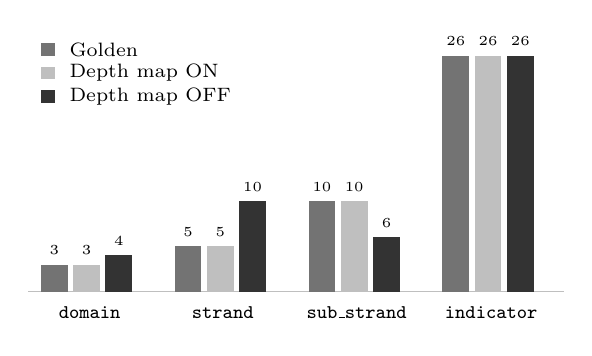
\begin{tikzpicture}[x=1cm, y=1cm]
\draw[gray!50] (0,0) -- (6.80,0);
\fill[black!55] (0.16,0) rectangle (0.50,0.346);
\node[font=\tiny, anchor=south] at (0.33,0.346) {3};
\fill[black!25] (0.57,0) rectangle (0.91,0.346);
\node[font=\tiny, anchor=south] at (0.74,0.346) {3};
\fill[black!80] (0.98,0) rectangle (1.32,0.462);
\node[font=\tiny, anchor=south] at (1.15,0.462) {4};
\node[font=\scriptsize, anchor=north] at (0.78,-0.06) {\texttt{domain}};
\fill[black!55] (1.86,0) rectangle (2.20,0.577);
\node[font=\tiny, anchor=south] at (2.03,0.577) {5};
\fill[black!25] (2.27,0) rectangle (2.61,0.577);
\node[font=\tiny, anchor=south] at (2.44,0.577) {5};
\fill[black!80] (2.68,0) rectangle (3.02,1.154);
\node[font=\tiny, anchor=south] at (2.85,1.154) {10};
\node[font=\scriptsize, anchor=north] at (2.47,-0.06) {\texttt{strand}};
\fill[black!55] (3.56,0) rectangle (3.90,1.154);
\node[font=\tiny, anchor=south] at (3.73,1.154) {10};
\fill[black!25] (3.97,0) rectangle (4.31,1.154);
\node[font=\tiny, anchor=south] at (4.14,1.154) {10};
\fill[black!80] (4.38,0) rectangle (4.72,0.692);
\node[font=\tiny, anchor=south] at (4.55,0.692) {6};
\node[font=\scriptsize, anchor=north] at (4.17,-0.06) {\texttt{sub\_strand}};
\fill[black!55] (5.26,0) rectangle (5.60,3.000);
\node[font=\tiny, anchor=south] at (5.43,3.000) {26};
\fill[black!25] (5.67,0) rectangle (6.01,3.000);
\node[font=\tiny, anchor=south] at (5.84,3.000) {26};
\fill[black!80] (6.08,0) rectangle (6.42,3.000);
\node[font=\tiny, anchor=south] at (6.25,3.000) {26};
\node[font=\scriptsize, anchor=north] at (5.88,-0.06) {\texttt{indicator}};
\fill[black!55] (0.16,3.00) rectangle (0.34,3.16);
\node[font=\scriptsize, anchor=west] at (0.40,3.08) {Golden};
\fill[black!25] (0.16,2.70) rectangle (0.34,2.86);
\node[font=\scriptsize, anchor=west] at (0.40,2.78) {Depth map ON};
\fill[black!80] (0.16,2.40) rectangle (0.34,2.56);
\node[font=\scriptsize, anchor=west] at (0.40,2.48) {Depth map OFF};
\end{tikzpicture}
\caption{Elements emitted per hierarchy level on Kentucky, whose detector golden is the corpus's only \emph{detection-exhaustive} one, with the depth-map pass enabled and ablated. With the pass enabled the detector reproduces the golden distribution exactly. Ablated, it emits an extra domain, doubles the strand count and loses four sub-strands, while the indicator count is untouched --- the failure is level \emph{collapse} at the two levels whose identity is positional rather than typographic. \textbf{This is not visible in a level-confusion matrix}: the evaluation matcher pairs on level, so an element emitted at the wrong level is recorded as a miss rather than an off-diagonal entry, and both arms render as clean diagonals. \texttt{\_only\_subset} corpus tier.}
\label{fig:levels}
\end{figure}


The mechanism is visible in Kentucky (Figure~\ref{fig:levels}), whose golden
annotates 3~domains, 5~strands, 10~sub-strands and 26~indicators. The on arm
reproduces that distribution exactly and the off arm emits 4, 10, 6 and 26.
Three repeated runs per arm show the same shape every time. Those repeats were
recorded at an earlier version of the detector code, before the Pass-1 sampler
was replaced, which is why I keep them distinct from the single-run columns of
Table~\ref{tab:ablation-depthmap}. In them the on arm reproduces the golden
distribution in all three, while the off arm inflates strand and deflates
sub-strand in all three (5~$\rightarrow$~8/7/10 and 10~$\rightarrow$~7/9/6) and
leaves the indicator count at 26. The failure is level \emph{collapse}, and it
is legible in the regression cases: with the map off, elements printed as
\texttt{Benchmark N.N} are promoted to strand, classified by their label rather
than by their position, which is precisely the behavior the method exists to
avoid.

Two qualifications. First, \textbf{the effect is conditional, not
uniform}: only Colorado and Kentucky lose recall, while Texas and Nevada keep
recall 1.000 and lose \emph{code} accuracy instead (Texas 8/8~$\rightarrow$~5/8
on an identical set of detections). Arizona and California are insensitive on
every metric, but that is an artifact of their goldens rather than a result:
both are small spot checks against far larger detection sets, so recall
saturates either way, and they are the states least able to show the effect.
Second, \textbf{off-arm recall is a range, never a point value}: across three
runs per arm per state at the earlier code version, Colorado spans 0.71--0.86
and Kentucky 0.89--0.98, and the recorded run at the current version (0.86 and
0.89) falls inside both ranges. The
direction never reverses in any sample, and the on arm is 1.000 with zero
variance across all eighteen runs, but the magnitude on any single run is a
draw. One regression case that failed at $n{=}2$ passed at $n{=}3$; I report it
as unstable rather than as evidence.

\subsection{Comparison: A Rule-Based Structure Extractor}
\label{sec:experiments-baseline}

To quantify what the language model contributes, I compare against a
rule-based structure extractor built on the cues such documents actually
provide: numbering patterns, capitalization, indentation and line shape. It is
graded by the same suite against the same goldens, through the same code path,
so the two columns are directly comparable. It was developed against the four
development states with the held-out pair untouched, and it carries no
per-document branch.

% AUTO-GENERATED by paper/analysis/generate_tables.py -- do not hand-edit.
% Source: paper/results/task4_20260823/baseline_comparison.json
% Regenerate with: python paper/analysis/generate_tables.py
% Corpus tier (guardrail 1): every row is the _only_subset tier, never full-document.
\begin{table*}
  \centering
  \begin{tabular}{lrrrrrrr}
    \hline
    & \multicolumn{2}{c}{\textbf{Recall}} & \multicolumn{2}{c}{\textbf{Raw precision}} & \multicolumn{2}{c}{\textbf{Code acc.}} & \\
    \textbf{State} & \textbf{LLM} & \textbf{Rule} & \textbf{LLM} & \textbf{Rule} & \textbf{LLM} & \textbf{Rule} & \textbf{Rule: found, wrong level} \\
    \hline
    AZ & 100.0 & 80.0 & 41.7 & 50.0 & 4/4 & 3/3 & 0/5 \\
    CA & 100.0 & 64.0 & 20.5 & 18.2 & 25/25 & 16/16 & 0/25 \\
    CO & 100.0 & 57.1 & 16.7 & 8.2 & 7/7 & 4/4 & 1/7 \\
    TX & 100.0 & 62.5 & 32.0 & 13.5 & 8/8 & 4/5 & 1/8 \\
    NV & 100.0 & 6.5 & 86.8 & 16.7 & 44/46 & 1/3 & 0/46 \\
    KY & 100.0 & 29.5 & 100.0 & 100.0 & 44/44 & 13/13 & 0/44 \\
    \hline
    \multicolumn{8}{l}{\emph{Pooled recall by level, all six states}} \\
    \hline
    domain & 100.0 & 100.0 & \multicolumn{5}{l}{LLM 13/13, rule-based 13/13} \\
    strand & 100.0 & 24.0 & \multicolumn{5}{l}{LLM 25/25, rule-based 6/25} \\
    sub\_strand & 100.0 & 66.7 & \multicolumn{5}{l}{LLM 24/24, rule-based 16/24} \\
    indicator & 100.0 & 13.7 & \multicolumn{5}{l}{LLM 73/73, rule-based 10/73} \\
    \hline
  \end{tabular}
  \caption{Rule-based baseline versus the LLM detector, graded by the \emph{same} suite against the \emph{same} goldens (Table~\ref{tab:detector-headline}). The baseline is document-agnostic: numbering depth, structural label words, ALL-CAPS and font-size cues from the bounding boxes, and column-aware reading order. It was developed against the four golden states only; NV and KY were first scored in the recorded run. \textbf{Raw precision is shown for both arms and is not a quality measure} except for KY, whose golden is detection-exhaustive: elsewhere it tracks annotation coverage, and it rewards under-emission, which is why the rule-based arm can exceed the LLM on AZ while finding fewer elements. Verified precision is not compared at all: the false-positive audit asks whether a title appears in the source text, and a rule-based extractor copies text rather than inventing it, so it scores near 1.000 by construction (\S\ref{sec:discussion-limitations}). A post-hoc probe widening two of the baseline's patterns to admit token shapes only the held-out documents use recovers NV 6.5\%$\rightarrow$52.2\%, KY 29.5\%$\rightarrow$40.9\%; the widenings are \emph{not} adopted, since they were motivated by the held-out set itself. Even repaired, the rule-based arm does not approach the LLM's recall. All numbers are on the \emph{\_only\_subset} corpus tier (8--15pp manually trimmed subsets), never full documents. Source: \texttt{paper/results/task4\_20260823/}.}
  \label{tab:baseline-comparison}
\end{table*}


\textbf{The per-level row is the result.} The rule-based arm ties the language
model exactly at domain (13 of 13 in both) and then collapses: strand
0.240, sub-strand 0.667, indicator 0.137, against 1.000 at every level. Reported
as a mean this would read ``1.000 versus 0.500'' and would hide the only thing
worth knowing. Typography identifies a document's top division in all six
states and identifies nothing reliably below it, because below the top division
the distinctions are positional.

The failure is also not the one I expected: elements the baseline misses are
overwhelmingly \emph{never emitted at all} rather than emitted at the wrong
level (43 of Nevada's 46 and 31 of Kentucky's 44). The rules do not mislabel
the structure so much as fail to see it.

\textbf{The held-out collapse needs its repair attached.} Nevada at 0.065 is the
most dramatic number in the table and the least trustworthy as stated: it is
dominated by a single token shape (\texttt{SS.ID.PK1}, a multi-letter code
segment) that none of the four development documents prints. Widening the
pattern after the fact recovers 0.522, and a comparable repair takes Kentucky
from 0.295 to 0.409. I adopt neither, because both were motivated by inspecting
held-out documents after the recorded run. The claim that survives the repair is
the one worth making: rules encode the shapes their author has seen, and even
generously repaired they reach roughly half the language model's recall on
documents they were not written against.

\textbf{Two cautions about the precision columns.} Raw precision is not a
quality ordering here: Arizona shows the rule-based arm \emph{above} the
language model (0.500 versus 0.417) purely because it emits fewer in-scope
detections against a five-element spot-check golden. I also omit verified
precision from this table deliberately. It asks whether a detected title
appears in the source text, a test for \emph{invention}, and an extractor that
copies verbatim cannot invent, so the baseline scores 1.000 in five of six
states against the language model's 0.9966. That number is real and
substantively backwards. Finally, the baseline has no Pass~1, so its depth-map
column reads \textsc{ablated} rather than failed, and it is deterministic, so
one run suffices.

\subsection{Comparison: A Single Whole-Document Prompt}
\label{sec:experiments-wholedoc}

The rule-based extractor of \S\ref{sec:experiments-baseline} answers what a
regular-expression approach cannot do. It does not answer the other obvious
question: why not hand the model the entire document in one prompt and read the
JSON back? \S\ref{sec:method-two-stage} argues against that; this measures it.
The arm is one call per document over the whole extraction, with no Pass-1 depth
map, no chunking and therefore no merge, and none of the deterministic repairs
of \S\ref{sec:method-parsing}. The prompt body, model, temperature, extractions
and grader are identical to the full method's, so a difference is attributable
to the architecture rather than to prompting.

\textbf{It is not a strawman: on Arizona and Nevada it matches}, at recall
$1.000$ with full code accuracy, and Nevada is one of the two held-out states
and prints a namespace that skips a level, so this is not an easy case. Where it
loses, it loses in two distinct ways. On Kentucky and Texas recall holds while
code accuracy falls, $44/44$ to $28/44$ and $8/8$ to $5/8$, and the failures are
precisely the repairs' absence: the model sampling its own abbreviation rule,
and codes left unanchored to their parents. Since a code composes the
identifier, each is a different primary key for the same standard. On Colorado
recall itself falls to $0.429$, with the level-collapse signature the depth-map
ablation produces.

\textbf{California is lost entirely, and that failure is architectural rather
than statistical.} Its single call emitted exactly 16{,}000 output tokens, the
configured maximum, truncating the JSON mid-object so that nothing parsed
and \emph{none} of its 25 golden elements were recovered, against $25/25$ for
the full method. One prompt has one output budget for an entire document, so
exceeding it loses the document; chunking bounds the same overflow to a chunk.
Arizona shows how narrow the margin is: it succeeded while emitting 14{,}292
tokens, within 11\% of the same ceiling, so a success here does not predict the
next document, and the margin is invisible in the score.

Scope bounds what this carries. Every subset extraction is between 3.7K and 7.9K
tokens and fits in one prompt, so a good score here would mean the architecture
is unnecessary \emph{at this tier} and would say nothing about the tiers where a
document does not fit and chunking is not optional. This arm is a single draw
per state, which is why I do not tabulate it; the California result is reported
with more confidence than the rest because its mechanism is identified rather
than inferred, the output length equaling the configured cap exactly. Source:
\texttt{task10\_20260905}.

\subsection{What the Confidence Score Measures}
\label{sec:experiments-confidence}

The detector emits a confidence score on every element, and nothing in the
pipeline thresholds it (\S\ref{sec:method-confidence}). This subsection reports
why I consider that the right decision rather than an oversight. The full
distribution, by state and by level, is
Table~\ref{tab:confidence-distribution} in
Appendix~\ref{sec:appendix-confidence}.

\textbf{The distribution is degenerate.} Across 379 elements the score takes
just five distinct values (0.90, 0.92, 0.95, 0.96 and 0.97), and 94.2\% of
them fall at 0.95 or above. The band the prompt explicitly reserves for a guess
($<0.70$) is never used once, and the whole of the range below 0.80 is empty. A
score that never exercises two thirds of the interval it was given is not
carrying much information about difficulty, and a review gate built on it would
mostly be a gate on noise.

\textbf{What variation there is tracks the document, not the difficulty of the
passage.} Three of the six states contain no sub-0.95 element whatsoever, and of
the 22 elements in the middle band, 16 belong to Kentucky alone; at indicator
level, 246 of 263 score 0.95 or above and all 17 exceptions come from two
states. Nor is the quantity stable between runs: on an earlier freeze of the
same corpus under the same configuration, 89.7\% of indicators scored 0.95 or
above against 93.5\% here, a four-point swing on an unchanged corpus, wider
than most of the distinctions a review threshold would be asked to draw.
Kentucky makes the point sharply, because it is the state I can say the most
about: its detector golden is the corpus's only exhaustive one, and against it
Kentucky achieves recall, code accuracy and verified precision of 1.000 while
carrying the lowest mean confidence of any state. Confidence separates Kentucky
from California; correctness does not.

\textbf{One observation that should not be over-read.} The single confirmed
hallucination in the corpus is also its lowest-scoring element, the only one
at 0.90, with nothing correct below 0.92, and it holds that position across
recordings. It is tempting to present this as a working detector for
fabrication. It is not one. There is exactly \emph{one} distinct invented
element in the audited corpus, so the false-negative rate of any such cut is
unmeasurable here; the threshold the prompt itself defines would catch nothing;
and the score is blind to the corpus's other non-verbatim category, since all 39
real-but-split titles, produced by column interleaving rather than by the model,
score at or above 0.95. I report the observation and decline to build on it.

\subsection{Stability: What Changes Between Identical Runs}
\label{sec:experiments-stability}

Every number reported so far is a single run of a sampling model, so the
question a reader should ask is how much of it survives re-running. I ran the
detector five times and the parser six times per state on identical frozen
inputs with caching disabled, deliberately split across two days.

% AUTO-GENERATED by paper/analysis/generate_tables.py -- do not hand-edit.
% Source: paper/results/task5_20260830/stability_analysis.json
% Regenerate with: python paper/analysis/generate_tables.py
% Corpus tier (guardrail 1): every row is the _only_subset tier, never full-document.
\begin{table}[t]
\centering
\small
\begin{tabular}{lrrr}
\toprule
& \textbf{ids} & \textbf{unstable} & \textbf{rate} \\
\midrule
\multicolumn{4}{l}{\emph{Detector}} \\
\quad AZ & 67 & 3 & 0.0448 \\
\quad CA & 51 & 0 & 0.0000 \\
\quad CO & 61 & 0 & 0.0000 \\
\quad TX & 33 & 0 & 0.0000 \\
\quad NV & 48 & 2 & 0.0417 \\
\quad KY & 44 & 0 & 0.0000 \\
\quad \textbf{pooled} & \textbf{304} & \textbf{5} & \textbf{0.0164} \\
\midrule
\multicolumn{4}{l}{\emph{Parser}} \\
\quad AZ & 45 & 0 & 0.0000 \\
\quad CA & 33 & 4 & 0.1212 \\
\quad CO & 48 & 0 & 0.0000 \\
\quad TX & 25 & 0 & 0.0000 \\
\quad NV & 24 & 5 & 0.2083 \\
\quad KY & 26 & 0 & 0.0000 \\
\quad \textbf{pooled} & \textbf{201} & \textbf{9} & \textbf{0.0448} \\
\bottomrule
\end{tabular}
\caption{Run-to-run stability, \textbf{\texttt{\_only\_subset} corpus tier}. Five detector runs and six parser observations per state, all \texttt{-{}-no-cache}, split across two days. \emph{ids} is the number of distinct element identities compared, \emph{unstable} how many differed in any graded field. \textbf{These rates are lower bounds, not estimates} (\S\ref{sec:experiments-stability}). Source: \texttt{paper/results/task5\_20260830/}.}
\label{tab:stability}
\end{table}


\textbf{The instability is concentrated rather than diffuse.} Four of six
states reproduce perfectly on each suite: California, Colorado, Texas and
Kentucky show zero detector disagreements across five runs, and Arizona,
Colorado, Texas and Kentucky zero parser disagreements across six. The movement
that exists is confined to three places, and each is a mechanism I can name.
Arizona's detector alternates on whether it emits three of its sub-strands
(present in four runs, absent in one), which changes output size without
touching any graded element. California's parser intermittently leaves the structural label inside
an indicator code, emitting \texttt{ELD.1.0.VOCA.Foundation 1.1.BROA} in two of
five comparisons. Nevada moves on both suites: a domain code that drifts between
the document's \texttt{S} and the domain's full name \texttt{Science}, and a strand
attachment that changes which of two headings three standards hang from.

\textbf{The California case is caught rather than stored.} All twelve of
those malformed codes contain whitespace, so the shape check at the validation
boundary (\S\ref{sec:method-parsing}) rejects every one before persistence. This
is the clearest evidence available that the check is load-bearing rather than
defensive decoration: the defect it was written for fires at a few percent per
run, and when it fires the records do not reach the database.

\paragraph{Why the runs were split across days.} Repeated runs inside one
session understate variance, and this measurement demonstrates it directly.
Nevada's detector emitted the same set of 54 elements in each of the three runs
executed in one evening (one of them differing only in the Science domain's
code), then dropped one indicator in \emph{both} runs executed the following
day. Five back-to-back runs would have reported that element as
perfectly stable.

\paragraph{A single run is not a safe basis for a claim, and I found that the
hard way.} An earlier recording of this system measured Nevada's detector code
accuracy at $46/46$ and I reported it as a held-out gain. It does not
reproduce: five fresh runs on identical code, the same extraction and the same
golden give $44$, $45$, $44$, $44$, $44$. Nevada's code accuracy is properly
reported as a \emph{range} of 44--45 of 46, and the earlier point value was the
top of its distribution rather than its center.

The same caution applied to a single-run ablation arm of my own, and repeating
it at $n{=}5$ per arm \emph{retired} the claim rather than confirming it. I had
attributed Nevada's two domain-code failures to the Pass-1 sampler on one draw
per arm; across five draws, one of those codes fails in \emph{every} draw of
\emph{both} arms, and at $n{=}1$ that arm had simply drawn the $46/46$ run
above. What survives is a rate rather than a cause: the layout-stratified
sampler gives mean code accuracy $0.965$ against the stride sampler's $0.935$,
its worst draw beating the stride sampler's best. But it also drops a golden
element in two draws of five where the stride sampler drops none, so it is
better on average and not better in every respect. Neither the sampler's
motivating evidence nor the depth-map ablation is affected: the first is a far
larger failure elsewhere, a four-level document reported as three
(\S\ref{sec:method-detection}), and the second is three runs per arm across six
states whose direction never changes sign.

\paragraph{What this does and does not license.} These rates are \textbf{lower
bounds, not estimates}. A defect firing in a minority of runs survives five
clean draws comfortably. The California defect above appears in two of five
comparisons, and an earlier investigation of a different parser defect, the
bare indicator code of \S\ref{sec:method-parsing}, found it in one graded run
of six within a single invocation and in ten of twenty cached runs across code
versions. A zero in Table~\ref{tab:stability} means I did not
observe instability at $n{=}5$, not that the component is deterministic. This is
why the table reports denominators beside every rate, and why the pipeline's
correctness argument rests on the validation boundary rather than on the model
agreeing with itself.

\subsection{Scale: the Batched Path on Multi-Batch Documents}
\label{sec:experiments-scale}

Every quality measurement above is computed at the \texttt{\_only\_subset}
tier, where each document produces at most five chunks and three domains. Both
batching layers therefore collapse to a single batch, the Step Functions
\texttt{Map} runs one iteration, and the merge is a no-op, so those tables,
whatever else they show, cannot support a claim about batching. This subsection
reports the one measurement that can.

% AUTO-GENERATED by paper/analysis/generate_tables.py -- do not hand-edit.
% Source: paper/results/task6_20260830/manifest.json
% Regenerate with: python paper/analysis/generate_tables.py
% Corpus tier (guardrail 1): every row is the _trimmed tier -- a document's standards content IN FULL (KY 52pp, CO 41pp) with non-standards matter removed. NOT the full published PDF (KY 120pp, CO 187pp), and NOT the _only_subset tier the quality tables use.
\begin{table}[t]
\centering
\small
\setlength{\tabcolsep}{4pt}
\begin{tabular}{lrr}
\toprule
& \textbf{KY} & \textbf{CO} \\
\midrule
Pages processed & 52 & 41 \\
\midrule
\multicolumn{3}{l}{\emph{Batching}} \\
Detection chunks & 18 & 17 \\
Detection batches & 4 & 4 \\
Parse batches & 9 & 9 \\
Elements, raw $\rightarrow$ merged & 363 $\rightarrow$ 329 & 390 $\rightarrow$ 300 \\
\midrule
\multicolumn{3}{l}{\emph{Input tokens}} \\
\quad Depth map & 12,153 & 19,613 \\
\quad Detection & 201,574 & 223,276 \\
\quad Parsing & 164,783 & 147,315 \\
\quad \textbf{Total} & \textbf{378,510} & \textbf{390,204} \\
\midrule
\multicolumn{3}{l}{\emph{Output tokens}} \\
\quad Depth map & 438 & 415 \\
\quad Detection & 64,530 & 47,125 \\
\quad Parsing & 85,205 & 83,862 \\
\quad \textbf{Total} & \textbf{150,173} & \textbf{131,402} \\
\midrule
LLM calls & 45 & 45 \\
Wall clock & 13m19s & 9m52s \\
\midrule
\multicolumn{3}{l}{\emph{Cost (USD)}} \\
\quad Depth map & \$0.0143 & \$0.0217 \\
\quad Detection & \$2.6211 & \$2.2945 \\
\quad Parsing & \$1.7724 & \$1.6999 \\
\textbf{Total} & \textbf{\$4.41} & \textbf{\$4.02} \\
\bottomrule
\end{tabular}
\caption{Batched-path scale, \textbf{\texttt{\_trimmed} corpus tier} --- each document's standards content \emph{in full}, and the only table here not at the \texttt{\_only\_subset} tier (\S\ref{sec:experiments-scale}). Each stage runs on the model assigned in \S\ref{sec:method-model-assignment}. \textbf{Tokens are the primary measure}; cost is derived from them at published Bedrock on-demand rates, recomputed at table-build time from the pipeline's own pricing constants. The depth-map pass is 0.3--0.5\% of a run's cost, detection 57--59\%. Source: \texttt{task6\_20260830}.}
\label{tab:scale}
\end{table}


\textbf{Table~\ref{tab:scale} is not the subset tier, and the distinction is
easy to misread in both directions.} These runs are the \texttt{\_trimmed}
tier: each document's standards content in full, with front matter, expository
essays and appendices removed. Kentucky's 52 pages are all of Kentucky's
standards, not 43\% of them. What the tier reduces is page count, and therefore
cost; it does not reduce coverage. Equally, these are not numbers for the
published PDFs, and the token and latency figures should not be extrapolated to
them.

At this tier the batching path is genuinely exercised: 18 and 17 detection
chunks resolve into four \texttt{Map} iterations per run, parsing into nine
batches, and the merge removes 34 and 90 duplicate elements respectively. A
no-op merge cannot remove 90 elements, so the reconciliation the architecture
performs is doing real work rather than passing data through.

\textbf{The stage breakdown is where the model-assignment principle of
\S\ref{sec:method-model-assignment} is tested.} Detection is the only stage
invoked once per chunk and accounts for 57--59\% of each run's cost. The
depth-map pass, the component the ablation above shows carries the
intermediate levels, runs once per document on the cheapest model and costs
between 0.3\% and 0.5\% of a run, about 1.4 cents on Kentucky and 2.2 on
Colorado. The most load-bearing
component in the method is very nearly the cheapest one, which is the outcome
the assignment was designed for.

Tokens are the primary measure and cost is derived from them at published
on-demand rates, recomputed at table-build time from the pipeline's own pricing
constants rather than transcribed by hand. Neither run was throttled, no
detection chunk returned empty, and the validator rejected no records, so these
figures describe a clean pass rather than a degraded one.

\subsection{Quality at Full-Document Scale}
\label{sec:experiments-scale-quality}

Every quality figure above is computed at the \emph{\_only\_subset} tier, and
the obvious objection is that subset-tier quality may not survive a whole
document: a larger run chunks further, and chunk boundaries are where a
detector can duplicate an element or lose one. \S\ref{sec:experiments-scale}
establishes that the batching path is genuinely exercised at the
\emph{\_trimmed} tier but grades nothing. This subsection grades it.

% AUTO-GENERATED by paper/analysis/generate_tables.py -- do not hand-edit.
% Source: paper/results/task13_20260907/ky_trimmed_3runs.json
% Regenerate with: python paper/analysis/generate_tables.py
% Corpus tier (guardrail 1): every row is the _trimmed tier -- a document's standards content IN FULL (KY 52pp, CO 41pp) with non-standards matter removed. NOT the full published PDF (KY 120pp, CO 187pp), and NOT the _only_subset tier the quality tables use.
\begin{table}[t]
\centering
\small
\setlength{\tabcolsep}{4pt}
\begin{tabular}{lrrrr}
\toprule
& \textbf{1} & \textbf{2} & \textbf{3} & \textbf{sd} \\
\midrule
\multicolumn{5}{l}{\emph{Detector} --- 277 verified elements} \\
\quad Elements emitted & 328 & 327 & 328 & 0.6 \\
\quad Absent from run & 0 & 0 & 0 & 0.0 \\
\quad Hallucinations & 0 & 0 & 0 & 0.0 \\
\quad Recall (level+title) & 1.000 & 1.000 & 1.000 & 0.000 \\
\quad Recall (strict key) & 0.592 & 0.588 & 0.592 & 0.002 \\
\quad Spurious \texttt{age\_band} & 164 & 164 & 164 & 0.0 \\
\quad Surplus duplicates & 51 & 50 & 51 & 0.6 \\
\midrule
\multicolumn{5}{l}{\emph{Parser} --- 207 verified standards} \\
\quad Standards parsed & 214 & 220 & 220 & \\
\quad Coverage & 0.807 & 0.927 & 0.841 & 0.062 \\
\quad Field accuracy & 0.997 & 0.994 & 0.994 & 0.002 \\
\quad Fabricated \texttt{.N} keys & 10 & 11 & 11 & 0.6 \\
\quad Collisions$^{\dagger}$ & 0 & 0 & 0 & 0.0 \\
\bottomrule
\end{tabular}
\caption{Quality at whole-document scale: Kentucky, three independent runs, \textbf{\texttt{\_trimmed} corpus tier} --- the document's standards content \emph{in full}, and not the \texttt{\_only\_subset} tier every other quality table uses (\S\ref{sec:experiments-scale-quality}). \textbf{Recall is measured against a verified reference set, not against the document}, so an element no run emits is invisible here (\S\ref{sec:discussion-goldens}). \textbf{Coverage is a range and must not be read as its mean.} $\dagger$~zero by construction: the resolver renames every collision before the check runs, so the informative count is the fabricated-key row above. Source: \texttt{task13\_20260907}.}
\label{tab:scale-quality}
\end{table}


\paragraph{Two measurements, and why the second was necessary.} The first
regrades the existing \emph{\_only\_subset} goldens \emph{inside} the
trimmed-tier run, translating page numbers through the recorded page map of
\S\ref{sec:corpus}. It needs no new annotation, and it isolates the variable
that matters: the same pages, the same golden, a larger neighborhood. Kentucky
and Colorado both come back with zero elements absent and zero ungrounded
detections. That measurement cannot speak to the rest of the document, so a
second one was built: both Kentucky trimmed-tier goldens are new (277
detected elements and 207 normalized standards, seeded from one recorded run
and then checked page by page against the published PDF), and three further
runs were executed and graded against them (Table~\ref{tab:scale-quality}).
Because the goldens were verified against a document rather than against the
run being graded, a miss is a real miss.

\paragraph{Detection recovers the whole reference set at scale.} All \textbf{277 of 277} verified
elements are found by all three runs. Not one is missed, and not one ungrounded
element is emitted, across a $6.5\times$ increase in page count and four
detection batches per run.

\paragraph{One field accounts for every anomaly.} Kentucky prints a
\texttt{THREE AND FOUR YEAR OLDS} banner at the head of each page. At the subset
tier the detector ignores it and every element comes back with a null age band,
matching the golden. At the trimmed tier it does not: 164 elements carry the
banner as their own \texttt{age\_band} in each of the three runs, with a
standard deviation of zero on the count, and 159 of those elements are the
same in all three runs (two runs agree exactly; the third differs on five). That
makes this a \textbf{systematic misreading rather than sampling noise}. Three
consequences follow, and together they are the entire difference between the
strict figures in Table~\ref{tab:scale-quality} and the ones above:

\begin{enumerate}
  \item elements fail the evaluation's matching key on that field alone, which
    is why strict recall reads $0.59$ while recall by level and title is
    $1.000$;
  \item \texttt{\_dedup\_elements} keys on \texttt{age\_band}, so the two
    spellings of one element never merge, and roughly 15\% of detector output
    survives as surplus duplicates;
  \item those duplicates collide in parsing and are separated by the
    identifier resolver's numeric fallback, so ten to eleven fabricated primary
    keys per run reach persistence, naming standards that do not exist.
\end{enumerate}

\textbf{Colorado is the control.} Its document has no age-band column and no
such banner, and in the same measurement it produces \textbf{zero} duplicates
and zero fabricated keys over 240 standards. That contrast is what makes the
attribution a measurement rather than a hypothesis.

\paragraph{Parser coverage is a range; parser field accuracy is not.} Coverage
spans twelve points across the three runs while field accuracy holds at $0.995
\pm 0.002$. The swing tracks the dropped-standard count exactly, and the
dropped standards are those the run assigned a narrower age band than the
document carries. \textbf{A single coverage figure for this document would be a
draw from that range}, and I report all three rather than their mean.

\paragraph{Two figures that look reassuring and are not.} Identifier collisions
are zero by construction: the resolver renames every collision before any
check runs, so the informative count is the fabricated keys above. And recall
here is measured \emph{against a verified reference set}, not against the
document: an element that no run emits is absent from the golden too, and
invisible to this measurement (\S\ref{sec:discussion-goldens}).

\paragraph{What this establishes.} Detection quality survives full-document
scale on the one document where it can be checked: complete recovery of a
verified reference set, no hallucination, in three independent runs. The
defects that scale introduces are concentrated in one field, are systematic
rather than random, and are documented rather than repaired, because the repair
changes a prompt and would invalidate every frozen measurement in this paper
(\S\ref{sec:discussion-limitations}). Source:
\texttt{task9\_20260905} and \texttt{task13\_20260907}.

\section{Discussion and Limitations}
\label{sec:discussion-limitations}

A deployed system's limits are the part of it a practitioner most needs, and
stating them precisely is the same discipline that produced the results above,
applied to the boundary of what I can claim. Where a limit is a measurement I
have not made, I say so; where it is one I made and did not like, I report it.

\subsection{What the results support}

The central claim survives its strongest available test. Classifying by nesting
position rather than by label vocabulary yields recall of 1.000 at every
hierarchy level in all six states, including the two held out entirely, whose
documents print label words, code namespaces and level counts that appear
nowhere in the four the prompts were written against, and neither of which is
special-cased anywhere in the system. The two comparisons locate that result
rather than merely asserting it, and they locate it at the same boundary from
opposite sides: ablating the depth map degrades exactly the levels whose
identity is positional and leaves the others untouched, while the rule-based
extractor matches the language model at a document's top division and collapses
beneath it. Typography identifies that top division reliably and identifies
almost nothing below it.

\subsection{Corpus scope, and what the tiers do and do not mean}

\textbf{Every headline quality number in this paper is computed at the
\texttt{\_only\_subset} tier}: roughly one to two domains per state, 70 pages
in total, hand-trimmed and exhaustively annotated. This is favorable
preprocessing and I state it rather than leaving it to be inferred. It is the
tier that makes annotation affordable, and it is a genuine reduction in
coverage: a subset metric is not a whole-document metric, and no table at that
tier should be read as one. The one exception,
\S\ref{sec:experiments-scale-quality}, grades whole-document runs against a
golden of its own and is kept in its own table.

The scale measurements are a different tier and a different kind of claim. They
run at \texttt{\_trimmed}, which removes only non-standards matter (front
matter, guiding-principles essays, appendices, acknowledgements) and
\textbf{retains every standard in the document}. Kentucky's 52 processed pages
are all of Kentucky's standards, not 43\% of them, and Colorado's 41 are the
complete Ages 3--5 publication. A trimmed-to-published page ratio is therefore
never a coverage fraction, and I am explicit about this because the opposite
reading is the more natural one and would understate the result.

What remains limited about scale is \textbf{page count, as a cost and batching
question rather than a coverage one}. These runs chunk 18 and 17 times across
four \texttt{Map} iterations; their token and latency figures should not be
extrapolated to untrimmed page counts, and no document as large as Arizona's
217-page publication has been run end to end. Trimming also remains
preprocessing that a deployment would have to perform or absorb: the pipeline
was never asked to ignore 68 pages of Kentucky preamble on its own, and I do
not claim it would. Colorado carries one further qualification. Its
out-of-scope content is other \emph{age bands}, the birth-to-three and five-to-
eight portions of a 187-page publication, not standards removed by trimming. Every
Colorado figure in this paper is the Ages 3--5 band.

\subsection{What the goldens can and cannot establish}
\label{sec:discussion-goldens}

The detector goldens vary a great deal in density, and that governs what each
can establish. In the four development states they are deliberate spot checks:
5, 25, 7 and 8 annotated elements against detection sets of 67, 122, 61 and
33. Because the evaluation suite counts every unmatched in-scope detection as a
false positive, \emph{raw} precision on those states largely measures annotation
coverage rather than detector quality, and I do not report it as quality.
Precision instead comes from a manual audit of all 297 in-scope detections
across the six subset-tier documents, which found a single hallucinated
element.

The two held-out states are annotated densely rather than as spot checks, and
they separate two properties that are easily conflated. Nevada's golden is
content-exhaustive (46 elements covering every distinct structural element
the document prints) but not \emph{detection}-exhaustive, because the
document reprints several headings on a second page spread and the detector
correctly finds them twice; at 46 golden against 52 in-scope detections its raw
precision has a ceiling below 1 no matter how well it performs. Kentucky's
golden is the one that is detection-exhaustive, 44 against 44, so its precision
is a genuine hallucination rate rather than a coverage figure. It is also, for
that reason, what made quality-at-scale evidence available without new
annotation: those 44 elements are graded inside a trimmed-tier run in
\S\ref{sec:experiments-scale-quality}.

\paragraph{The trimmed-tier goldens support precision and not recall, and the
distinction is not a technicality.} The two Kentucky goldens used at that scale
(277 elements and 207 standards) were produced by seeding each row from a
recorded run and then checking it against the published PDF. Verifying emitted
rows establishes that what the system produced is correct, which is a precision
claim. It cannot establish recall, because it never searches for what the system
\emph{omitted}: an element no run emits is absent from the golden as well, and
invisible to any measurement made against it. Recall at that scale is therefore
reported against a verified reference set of 277 elements rather than against
the document, and the ceiling travels with the number wherever it appears.

Independent evidence bounds the gap at the middle levels without closing it.
Every distinct \texttt{Benchmark N.N} identifier the document prints (18 of 18)
and every \texttt{<Domain> Standard N} heading (15 of 15) appears in the golden,
recovered from the document text rather than from any run. The 202 indicators
carry no equivalent check, and that is where an omission would hide. Closing it
needs a cold read of the pages, reading a random sample without reference to
the golden and diffing, which would cost a fraction of annotating the document
and is the obvious next measurement.

\paragraph{Colorado deliberately carries only half of this.} Its golden remains
a seven-element spot check and is not being extended, so at the trimmed tier it
contributes recall and duplication evidence (zero elements absent, zero
duplicates, across four detection batches on the corpus's hardest layout) and
no precision figure at all. Its raw precision there is an annotation-coverage
artifact and is labeled as one in the recorded output. The corpus therefore has
exactly one state whose precision is a quality figure, at either tier, and that
is a real limit on how far the evidence generalizes.

\subsection{Nondeterminism, and why I do not claim determinism}

The pipeline is not deterministic, and the stability measurements should be read
as \textbf{lower bounds rather than estimates}. A defect firing in a minority of
runs survives five clean draws comfortably, so a zero in my stability table
means I did not observe instability at $n{=}5$, not that a component is stable.

Two of my own recorded results are the cautionary cases, and
\S\ref{sec:experiments-stability} reports both: a held-out code accuracy of
$46/46$ that five fresh runs give as 44, 45, 44, 44, 44, and a single-draw
attribution of Nevada's domain-code behavior to the Pass-1 sampler that $n{=}5$
per arm retired rather than confirmed. Both were the top of a distribution read
as its center. Where an experiment is repeated (the depth-map ablation, at
three runs per arm across six states) I report the range and note that the
direction never reverses, rather than quoting a single number.

The practical consequence is that correctness here rests on the validation
boundary rather than on the model agreeing with itself. The clearest instance is
California's intermittent structural-label defect: when it fires it produces
twelve malformed identifiers, all of which contain whitespace and are rejected
on shape before persistence.

\subsection{A known defect, measured and deliberately not repaired}
\label{sec:discussion-ageband-defect}

\S\ref{sec:experiments-scale-quality} reports that one field accounts for every
anomaly the trimmed tier introduces: the detector attributes a page banner to
individual elements, which defeats the deduplication key, which produces
duplicate standards, which the identifier resolver separates with fabricated
suffixes. I know the cause, I know the fix, and I have not applied it.

The fix is a prompt rule stating what the goldens already encode across all six
states: that an element's age band comes from a side-by-side column that
distinguishes it from its siblings, never from a banner or running header that
applies to a whole page. That is a general document-structure principle rather
than a per-state rule, so it belongs in the prompt by the discipline of
\S\ref{sec:method-llm-first}. Applying it changes a prompt, which changes the
hash that every recorded measurement in this paper is keyed to, and would
require re-recording the headline, ablation and comparison arms.

I report the defect rather than repair it, and state the reason plainly: the
cost of the repair is the invalidation of the evidence. That is the same
cost-gating that governs every other change to these two files, applied to a
finding of my own, and a reader is entitled to weigh it. Two things make the
deferral defensible rather than convenient. The defect does not affect any
subset-tier number, where the banner is not attributed at all. And it is
systematic rather than random: the count is 164 in each of three consecutive
runs, and 159 of those elements are common to all three, so its effect is
bounded and reproducible rather than a source of unquantified noise.

\subsection{Limitations of the measuring instruments}

Three are worth stating because each could mislead a reader who assumed
otherwise.

\textbf{The false-positive audit tests for invention.} Its verdicts turn on
whether a detected title appears in the source text, which is the right question
for a generative system and the wrong one for a copier: a rule-based
extractor cannot invent and therefore scores near 1.000 by construction. Applied
to the baseline the metric also detects something other than hallucination:
California's five flagged rows are column \emph{fusion}, where a table header
has been merged into an adjacent title, rather than fabrication. I report raw
precision for both arms instead, and treat the audit as informative only about
the language-model arm.

\textbf{The two evaluation suites do not grade the same detection.} The detector
suite re-runs detection in process against a frozen extraction (the direct
path) while the parser suite grades the deployed batched path's stored
output. On the recording this paper uses, Arizona's direct-path detection holds
67 elements where the batched output the parser suite reads holds 65; earlier
recordings have differed by more. The two suites also use
independently annotated goldens with different shapes, a flat element list and
nested normalized records. A detector number and a parser number from the same
results directory therefore describe related but not identical objects, and
should not be composed into a single end-to-end figure.

\textbf{Extraction quality bounds everything downstream.} The pipeline reads OCR
and PDF text-layer output; a heading the extractor fuses or drops is not
recoverable by any amount of downstream reasoning. Nevada's one confirmed
hallucination originates this way, in a multi-column table that flattens into
interleaved reading order.

\subsection{Scope}

The corpus is six US states of more than fifty jurisdictions, all in English,
all early learning standards. I make no claim about other document families,
other languages, or other countries' standards traditions, though the method
assumes only that a document has a nesting structure and prints some evidence
of it. Neither code nor corpus is released (\S\ref{sec:artifacts-statement}):
the source documents are third-party state-agency publications that are not ours
to redistribute, which limits direct reproducibility to the prompts and schema
disclosed in the appendices.

\section{Conclusion and Future Work}
\label{sec:conclusion}

US early learning standards are public policy that software cannot read. I have
shown that the obstacle is not text recovery but hierarchy recovery, and that an
LLM can recover the hierarchy by classifying each element's nesting position
against a depth map inferred per document, rather than by recognizing label
vocabulary that no two states share. Across four development states and two held
out entirely, detector recall at the annotated subset tier is 1.000 at every
level, a manual audit of all 297 in-scope detections there finds one
hallucinated element, and parsing resolves those
elements into a single canonical schema with no identifier collisions. Ablating
the depth map degrades exactly the levels whose identity is positional and
leaves the others untouched; a rule-based extractor matches the method at a
document's top division and collapses beneath it. The system carries no
per-state code path, which is what allows a new state to be added without new
code; the prompts' worked examples are the one place the corpus's own documents
appear, and they are itemized rather than left implicit.

Quality at full-document scale, which an earlier draft named as the measurement
this work most conspicuously lacked, is now reported: on Kentucky's trimmed tier
all 277 elements of a verified reference set are recovered in each of three
independent runs, with no hallucination, and parser field accuracy is $0.995$.
What that leaves is a bounded and stateable gap rather than an absence --- the
reference set was verified by inspecting what the system emitted, so it
establishes precision and not recall, and a cold read of a random sample of
pages is the cheap way to close it. Beyond that, the corpus is six states of
more than fifty, and the obvious direction is breadth: each state added tests
generalization again, and enough of them would constitute the national
machine-readable dataset that does not currently exist.

Two further directions follow from the artifact rather than the method.
Exposing the normalized store through a tool-callable interface would let
external applications query standards directly, which is the form curriculum
and planning tools need them in. And the per-element verification state invites
a targeted-review question I have deliberately not answered: given that
confidence is uninformative (\S\ref{sec:experiments-confidence}), what
\emph{would} identify the records most worth an expert's attention? My
stability measurements suggest one candidate --- disagreement across repeated
runs is cheap to compute and, unlike confidence, is concentrated in exactly the
places where my own defects live.

% ethics.tex — Task 10 stub. Outline recovered verbatim from the original
% plan file fragment (see ../OUTLINE_NOTES.md). Draft at Task 12.
%
% Education-data stewardship, human verification, no student data.

\section{Ethics and Broader Impact}
\label{sec:ethics}

\section{Artifacts Statement}
\label{sec:artifacts-statement}

Neither the implementation nor the evaluation corpus is released. Disclosure is
in-paper: the appendices give the detector and parser prompts
(Appendix~\ref{sec:appendix-prompts}, with their complete unabridged text
shipped alongside this paper as the ancillary file \texttt{anc/prompts.txt}),
the canonical schema
(Appendix~\ref{sec:appendix-schema}), representative annotated examples
(Appendix~\ref{sec:appendix-goldens}), and the corpus table naming every source
document with its publisher, year and retained page ranges
(Appendix~\ref{sec:appendix-corpus}). Those are the parts a reader needs to
evaluate or reimplement the method; the rest is engineering around them.

The source documents are third-party state-agency publications. Only US
\emph{federal} works are automatically in the public domain, so these are not
ours to redistribute, and the corpus appendix cites each document's origin so it
can be obtained from its issuing agency instead. The hand-annotated golden sets
are derived from those documents and are withheld for the same reason.

I state the consequence plainly: this limits direct reproducibility. A reader
can reimplement the method from the prompts and schema and apply it to documents
they obtain themselves, but cannot re-run my exact measurements. To make the
reported numbers as checkable as the constraint allows, every result in this
paper is generated from a recorded JSON artifact rather than transcribed by
hand, each carries the pipeline source version and model identifiers that
produced it, and each table is regenerated from those artifacts at build time.
Every table caption names the artifact behind it by task and recording date
---~\texttt{task8\_20260904}, say~--- and those recordings are retained and
available on request; the date is load-bearing, because several measurements
were re-recorded when the code version moved and the tag is what distinguishes
one freeze from another. Where a figure could not be verified against an
authoritative source I say so rather than reporting it.

This paper is distributed under the arXiv non-exclusive license to distribute.
Copyright is retained by the author; no redistribution or derivative use of the
text is granted.


% Bibliography: paper/references.bib (Task 9 deliverable). Task 13 keeps the
% compiled .bbl and deletes the .bib from the arXiv tarball.
\bibliography{references}

\appendix

\section{Prompts}
\label{sec:appendix-prompts}

% AUTO-GENERATED by paper/analysis/make_prompt_appendix.py -- do not hand-edit.
% Rendered from the live prompt builders so the appendix cannot drift from the
% implementation it discloses. Regenerate with:
%   python paper/analysis/make_prompt_appendix.py

The three prompts below are reproduced as the system emits them, with only the
per-run document content replaced by a placeholder. Together with the schema of
Appendix~\ref{sec:appendix-schema} they are what this paper discloses in place of
a code release (\S\ref{sec:artifacts-statement}).

\subsection{Pass 1: depth-map inference}
\label{sec:prompt-depthmap}
\begin{lstlisting}[style=promptstyle]
You are analyzing the structural skeleton of an early learning standards document. You will NOT extract individual elements — only the document's nesting hierarchy.

Read the sample below and identify how many distinct nesting depths the document uses, what each depth looks like (its prefix/label pattern), and one concrete example. The DEEPEST depth is always the leaf (individual learning goals/foundations/benchmarks).

This document's depths must then be mapped to a canonical 4-level hierarchy:
- depth 1 → "domain"
- depth 2 → "strand"
- depth 3 → "sub_strand"
- deepest depth → "indicator"

Rules:
- Fill the canonical levels FROM THE TOP DOWN. The first depth is always "domain", the deepest depth is always "indicator", and any depth in between takes the next canonical level in order: the depth directly under domain is "strand", the one below that is "sub_strand". A document with fewer depths therefore drops the levels at the BOTTOM of that middle range — never "strand".
- A 4-level document (domain > group > sub-group > leaf) maps to: domain, strand, sub_strand, indicator.
- A 3-level document (domain > group > leaf) maps to: domain, strand, indicator. There is NO sub_strand — the single middle level is a STRAND, never a sub_strand.
- A 2-level document (domain > leaf) maps to: domain, indicator. There is no strand and no sub_strand.
- Use depth POSITION, not the document's labels. If a document uses "Sub-Strand" as the label for the second level (directly under domain), it is still a STRAND in our canonical hierarchy — and likewise a document that calls its single middle level "Section", "Concept", "Goal", or anything else still maps that level to "strand".

Every line is prefixed with its page and the horizontal position it was laid out at: `[Page N | x=0.09]`, where x is the line's left edge as a fraction of the page width. Use x to work out whether a page uses a side-by-side layout: lines of one column share nearly the same x, and a jump to a clearly different x means a different column. Lines you judge to be in the same column read as one continuous cell, even when lines from other columns are interleaved between them. Treat parallel columns as repetitions of ONE depth, not as separate depths.

Be deterministic and conservative. Do not speculate. If you cannot tell whether two depths are distinct, assume they are the same depth.

Output ONLY a JSON object with this exact shape:
{
  "doc_depths": [
    {"depth": 1, "canonical_level": "domain",     "label_in_doc": "<what the doc calls this>", "prefix_pattern": "<regex-ish pattern e.g. 'ALL-CAPS HEADING' or 'N. <Title>: <desc>'>", "example": "<exact text from doc>"},
    {"depth": 2, "canonical_level": "strand|indicator", ...}
  ],
  "notes": "<one short sentence about the LEVEL LAYOUT only, e.g. 'age-band columns repeat one depth'. A later stage reads this as an instruction, so: never describe text below the deepest depth as examples/illustrations/anecdotes, and never say to ignore or skip anything. Empty string if nothing unusual.>"
}

DOCUMENT SAMPLE:

<<serialized document lines, one per row, each prefixed
  [Page N | x=<left edge as fraction of page width>]>>
\end{lstlisting}

\subsection{Pass 2: per-chunk detection}
\label{sec:prompt-detection}
\begin{lstlisting}[style=promptstyle]
You extract structural elements from an early learning standards document chunk.

Be deterministic. Be conservative. Do not be creative. Two runs over the same text MUST produce the same JSON. Do not invent titles, codes, or descriptions — only use text that literally appears in the chunk.

CANONICAL HIERARCHY: domain (1) > strand (2) > sub_strand (3) > indicator (leaf). A document with fewer levels drops them from the BOTTOM of the middle: the level directly under domain is always `strand`, and `sub_strand` exists only when there are two levels between domain and the leaf. So a 3-level document is domain > strand > indicator, never domain > sub_strand > indicator. The depth map says which levels exist.

LAYOUT COORDINATES: every line is prefixed with its page and the horizontal position it was laid out at — `[Page N | x=0.09]`, where x is the line's left edge as a fraction of the page width (0.00 is the left margin, 1.00 the right). Use x to work out the page's column structure yourself: on a side-by-side layout the lines of one column share nearly the same x, and a jump to a clearly different x means a different column. Lines you judge to be in the same column must be read together as one continuous cell, in the order given, even when lines from other columns are interleaved between them. Never join text across what you judge to be two different columns into a single element, and never attribute one column's prose to another column's element. Expect a header that spans the whole layout to sit at the leftmost x while belonging to every column beneath it. A line tagged only `[Page N]` has no usable coordinate; use the text's own layout cues there.

CLASSIFICATION RULE:
- If a depth map is provided, look up each element's depth in the document and use the `canonical_level` from that depth. Do NOT reclassify based on prefix style.
- If no depth map is provided, classify by nesting POSITION, never by what the document calls a level.

EXTRACTION RULES:
1. Emit every structural element you see, even if its children are not in this chunk. Emit ONLY what you see: every element must be backed by a heading line that literally appears in this chunk, and its `title` must be text copied from that line. A position identifier you read inside a CHILD's code is NOT evidence that the parent's heading is present. A child code names its ancestors — an indicator coded `A.B.2.c` says it sits under the `2` at the level above — but that tells you only where the child belongs; it does not put the parent's heading on the page. When a chunk opens part-way through a section and an ancestor's heading was left behind in the previous chunk, emit the children alone and leave the ancestor out. A later chunk that contains the heading will supply it, and the parent is reconstructed downstream from the children's codes. Never reconstruct it here by reading the code apart. Emit ONLY what you see: every element must be backed by a heading line that literally appears in this chunk. (This says only that the heading must BE there — how you split that line into `title`, `code`, and `description` is decided by rules 4 and 8 as usual, and this rule never tells you to copy the whole line into `title`.) A position identifier you read inside a CHILD's code is NOT evidence that the parent's heading is present. A child code names its ancestors — an indicator coded `A.B.2.c` says it sits under the `2` at the level above — but that tells you only where the child belongs; it does not put the parent's heading on the page. When a chunk opens part-way through a section and an ancestor's heading was left behind in the previous chunk, emit the children alone and leave the ancestor out. A later chunk that contains the heading will supply it, and the parent is reconstructed downstream from the children's codes. Never reconstruct it here by reading the code apart.
2. A lettered/bulleted list (a., b., c., …) is EITHER the leaf indicators OR illustrative examples below a leaf — decide using the depth map, never the "a./b." surface style:
   - If the document's DEEPEST depth in the depth map is this lettered list (i.e. there is no deeper indicator level beneath the letters), then EACH lettered item IS an indicator. Emit one indicator per letter. Its `title` is the lettered item's own skill/competency statement (the text after the letter, e.g. "a. Demonstrates self-confidence." → "Demonstrates self-confidence"); any further example anecdotes indented beneath that letter go in its `description`. Do NOT fold these letters away and do NOT drop them — every lettered item in the chunk must appear.
   - Otherwise (the letters sit BELOW an already-identified leaf indicator and read as concrete behavior anecdotes, not skill statements) they are an EXAMPLE LIST — see rule 2a. Do NOT emit them as separate indicators.
2a. EXAMPLE LISTS — decide by OWNERSHIP, not by how illustrative the text sounds. This applies only to text the depth map does NOT place at a structural depth; anything at a depth is an element (rule 2) and is emitted regardless of how example-like it reads. For the remaining, non-structural text, find the run's owner with this exact two-step test, in this order:
   STEP 1 — Find the ANCHOR. Scan UPWARD from the run's first line and stop at the very first line that the depth map places at a structural depth. That element is the ANCHOR. Its depth is irrelevant: the anchor is the NEAREST element above the run, never the section's top-level heading. A leaf indicator is an anchor exactly like a domain or strand is — including a lettered item that rule 2 made an indicator.
   STEP 2 — Look ONLY at the lines lying strictly BETWEEN the anchor and the run. Nothing above the anchor is part of this test.
   - A heading or lead-in line lies in that gap — a non-structural line that names the run as a category rather than asserting a requirement ("Child Behaviors", "Examples", "The child may:", "For example:"). That line owns the run, and it is a section label rather than a structural element, so NOTHING from the run is extracted: do not emit the lead-in, do not emit the entries, and do NOT copy the entries into the anchor. The anchor's `description` keeps only its own prose, which is often absent — write `null` then. The same holds for a run laid out full-width BENEATH side-by-side columns: it is owned by no single column, so it enters no column's `description`.
   - The gap is empty — the run simply continues directly underneath the anchor. Then it IS the anchor's own text, however anecdotal or example-like it reads. Put it in the anchor's `description`, verbatim. Never discard text merely because it illustrates: discard it only when the document has given it somewhere else to belong. Being CALLED an example is not being given somewhere else to belong — not by the depth map's `notes`, not by a section header higher up the page, not by your own reading of the tone. Only a lead-in sitting in the gap does that.
   A heading's claim is SPENT the moment a structural element appears beneath it. A section header followed by structural elements is a label for that GROUP and hands ownership DOWN to them; it never reaches past them to claim text nested under one of them. This holds even when the header's own wording announces examples — a header that names both the indicators and their examples still owns nothing itself, and each indicator beneath it owns the example lines nested under that indicator.
   Either way, such a run is never promoted to elements of its own.
3. Side-by-side age-band columns: emit ONE element PER column. Different age bands = different indicators, even when they share a code stem and title. Set `age_band` to the column label (e.g. "Early (3 to 4 ½ Years)", "PK3", "By 36 months"). Strip the age-band label from `title`. Put only that column's prose in `description`. If a row shows N age columns it MUST yield exactly N indicators — emit EVERY column even when a column's prose is short, nearly identical to its neighbor, or visually sparse. Never collapse or skip a column.
   - Spell each age-band label identically every time, using the document's exact glyphs (write "½", not "1/2").
4. `code`: REQUIRED on every element you emit. It is NEVER `null`, never an empty string, and the key is never omitted — an element without a code cannot be stored, and emitting one costs us the whole chunk it sits in. If the document prints no code for the element, the abbreviation procedure at the end of this rule ALWAYS supplies one; that is precisely what it is for, so "uncoded" is never a reason to answer `null`. The `ABSENCE IS null` instruction in rule 8 governs `description` and nothing else — it does NOT apply to `code`. Now: use the document's code if present. Before you decide none is present, LOOK for it — a document often prints an element's code somewhere other than on its heading line, and a code you can RECOVER from the page ALWAYS beats one you would derive from the title. Search these three places, in this order, and stop at the first that yields a code:
   (i) ON THE HEADING LINE — a code printed inline with the title ("1.0", "I.A.2", "PK3.I.A.2"), including the `<Label> <id>` form described in the bullets below. This always wins: an element that prints its own id keeps it, even when its descendants' codes are built on a different stem.
   (ii) IN A CAPTION BESIDE THE HEADING — a code the document prints just above, below, or beside the title rather than on it: inside parentheses, on a small caption line, in a table or column header, or in a lead-in that names the group of items which follows. A heading "Working Memory" whose next line reads "Indicators (CD.WM)" has code "CD.WM". Take only the IDENTIFIER — the caption's surrounding words ("Indicators", "Standards", "Codes") name what the caption points at and are not part of the code — and copy it VERBATIM, dots included.
   (iii) FROM ITS DESCENDANTS' CODES — the heading prints no code of its own anywhere, but the elements BENEATH it carry dotted codes that all begin with the same segments. An ancestor's code is the COMMON PREFIX of its descendants' document codes. Indicators coded "CD.WM.PK1", "CD.WM.PK2", "CD.AT.PK1", "CD.AT.PK2" say that the group heading above the first two is "CD.WM", the group above the last two is "CD.AT", and the level above all four is "CD". Emit the WHOLE shared prefix with its dots ("CD.WM") — never just its last segment ("WM"), and never an abbreviation of the title.
       Peel exactly ONE segment per level as you move UP, so a recovered prefix never reaches past the level directly below it: the parent of an indicator coded "CD.WM.PK1" is "CD.WM", and the level above THAT is "CD". A level that prints its own code under (i) takes that code and consumes NO segment — keep peeling from where you were for the level above it. Peel this way even when the chunk happens to show only one group under a heading, where the raw shared prefix would over-reach ("CD.WM" for a level that is really "CD").
       Take a prefix only when the evidence is real:
       - The descendant's code must have MORE THAN ONE dot-separated segment. A single-segment code ("1", "a", "VOCA") names only the element itself and holds no ancestor inside it.
       - At least TWO descendants must agree on the prefix AND differ after it. One descendant alone cannot show where its code stops naming ancestors and starts naming itself.
       - Only WHOLE segments count. Never split a segment.
       - A descendant code that carries a structural LABEL word ("Foundation 1.7", "Benchmark 1.1", "Standard 2") is NOT a namespace path: the label names that descendant's OWN level, so the entire id after the label belongs to the descendant and none of it is an ancestor's code. Take a prefix only from bare dotted codes ("CD.WM.PK1", "I.A.2").
       This rule decides WHICH code an element gets. It NEVER licenses emitting an element you cannot see — rule 1 still governs that, and the heading line must literally appear in this chunk. If it does not, emit the descendants alone and take nothing from them.
   When (ii) or (iii) supplied the code, cite the line it came from in `source_text` IN ADDITION to the heading line — that line is part of the text you used (rule 7). Never instead of the heading line: rule 1's self-check still holds, and if a descendant's line is the ONLY line you can cite, you did not see the heading and must not emit the element at all.
   ONLY when all three come up empty — the document leaves this element genuinely uncoded — do you generate a stable ≤5-char uppercase abbreviation from the title, by this EXACT procedure:
   (a) Split the title into words on spaces and slashes. A hyphenated compound is ONE word ("self-selected" → one word contributing "S"; "Health/Mental Wellness" → three words).
   (b) DROP every CONNECTOR word. A connector is any of: `a an the and or but nor of to in on at by for from with into about over under through as`, and the symbol `&`. Connectors carry no meaning in a code — their initials only crowd out the words that do, and the code has just 5 characters to spend. Keeping them yields a code made of function words: "Attends to an adult or peer who is communicating verbally or nonverbally" would give "ATAAO" ("Attends To An Adult Or") instead of "AAPWI", and "Engages in an activity for a sustained period of time" would give "EIAAF" instead of "EASPT". The code is the human-readable part of a standard's identifier, so it must spend its characters on the words that name the skill. This list is exact — do not extend it to other prepositions you may consider connector-like ("toward", "during", "between", "despite", "while"): those are CONTENT words for this purpose and their initials stay in the code. Match case-insensitively and ignore trailing punctuation.
   (c) If exactly ONE content word remains, the code is its first 4 letters ("Vocabulary" → "VOCA", "Initiative" → "INIT"). Otherwise the code is the first letter of each remaining content word, in order, capped at the first 5 ("Physical Development" → "PD", "Approaches to Learning" → "AL", "Concepts About Print" → "CP", "Social & Emotional Development" → "SED", "Language and Early Literacy" → "LEL", "Engages in an activity for a sustained period of time" → "EASPT").
   (d) If dropping connectors would leave NO words at all, keep the title's words as they are and apply (c) to those.
   Use the SAME code every time the same element appears.
   - When a heading is written as `<Label> <id>: <Title>` — where `<Label>` is ANY structural word the document uses to name a level (e.g. Strand, Concept, Sub-Strand, Goal, Pillar, Unit, Theme, Section, Element, Standard, Domain, Benchmark, Component, Cluster, Foundation, Outcome, or whatever else this particular document uses) and `<id>` is the position identifier at that level (a number "1", a letter "A", a token "1.2") — the label-plus-id together is the element's `code`, written as the label, ONE space, then the id (e.g. "Strand 1", "Concept 2", "Goal A", "Pillar 1.2"). Whatever punctuation the heading used to separate the label from the id — a colon, hyphen, en/em dash — is layout and does NOT enter the code: "Strand: 1.0 — Listening and Speaking" gives code "Strand 1.0", never "Strand: 1.0". The `title` is ONLY the text after the colon (e.g. "Strand 1: Self-Awareness and Emotional Skills" → title "Self-Awareness and Emotional Skills"). This rule applies to EVERY structural-label heading word, not just the examples — never leave the `<Label> <id>:` prefix inside `title`, regardless of which word the document chose for `<Label>`.
   - A structural label word contributes NOTHING to the code on its own. It earns a place in the code only through the position identifier attached to it: "Strand 1" works as a code because "1" says WHICH strand. So when a heading names the level but supplies no position identifier — `<Label><separator><Title>` with nothing between the label and the title, whatever the separator (colon, hyphen, en/em dash, or just a space): e.g. "Sub-Strand — Vocabulary", "Concept - Curiosity and Interest", "Domain: Number Sense", "Goal — Working Memory" — the label is pure level-naming, exactly like the trailing structural noun below. Drop it and derive the code from the TITLE ALONE using the ≤5-char abbreviation rule ("Vocabulary" → "VOCA", "Curiosity and Interest" → "CI", "Number Sense" → "NS", "Working Memory" → "WM") — unless the document supplies a code for the element somewhere else, in a caption or through its descendants' codes, in which case that recovered code wins over any abbreviation ((ii)/(iii) above). Never abbreviate the label into the code and never prefix the code with it ("Sub-Strand — Vocabulary" → "VOCA", NOT "SS-V"; "Concept - Curiosity and Interest" → "CI", NOT "C-CI"), and never use the raw heading line as the code.
   - The same principle holds when the structural label appears as a TRAILING noun on the heading instead of a prefix: a heading like `<Title> <Label>` (e.g. "Social and Emotional Development Domain", "Language and Literacy Standard", "Physical Development Area", "Number Sense Strand") names a `<Title>` of a level the document calls `<Label>`. The structural noun is the level word, NOT part of the name — emit only the bare `<Title>` ("Social and Emotional Development", "Language and Literacy", "Physical Development", "Number Sense"). This applies regardless of which structural noun the document uses (Domain, Standard, Area, Strand, Section, Component, Cluster, Foundation, etc.). The same-named element may also appear elsewhere on the page as a running page header in ALL CAPS (e.g. "SOCIAL EMOTIONAL DEVELOPMENT STANDARD" repeated at the top of every page) — that running header is page typography, not a separate element and not a code; if you emit anything for it, normalize it back to the same bare title-cased `<Title>` so the two variants share the SAME `code` and the SAME `title`. The abbreviation rule above ("≤5-char uppercase abbreviation from the title") still applies WHEN the document leaves the element uncoded: derive the code from the BARE title (e.g. "Social Emotional Development" → "SED"), NEVER use the heading text itself or the structural noun as the code. If the document DOES code it — in a caption, or through the shared prefix of its descendants' codes — that recovered code wins ((ii)/(iii) above).
   - When a lettered list IS the leaf indicators (per rule 2), the `code` is JUST that item's letter, lowercased ("a", "b", "c", …) — exactly as the document orders them, regardless of any OCR casing. Do NOT prepend the parent strand/concept number (no "S1C1a"), and do NOT uppercase it (no bare "C"). The downstream parser supplies the parent's number; the detector only needs the consistent local letter.
5. `confidence`: 0.95+ if the depth map clearly applies; 0.80-0.94 if the chunk is ambiguous but the answer is likely; <0.70 if you are guessing.
6. `source_page`: page number from the `[Page N]` / `[Page N | x=…]` marker on that line.
7. `source_text`: the exact line(s) from the chunk you used. Copy verbatim, WITHOUT the leading `[Page N]` / `[Page N | x=…]` marker.
8. `description`: capture the element's COMPLETE descriptive/introductory prose, verbatim — EVERY sentence of a domain/strand/sub_strand introduction that appears in the chunk, not just the first sentence. Do NOT summarize, paraphrase, shorten, or stop at the first sentence. If the intro runs across several sentences or lines in the chunk, include all of them. (For an age-band column indicator, `description` is still only that one column's prose, per rule 3.) `description` holds only the text the element OWNS (rule 2a) — never a run that a heading or lead-in of its own has claimed; an element that owns no prose gets `null` for `description`, and that is the correct answer, not a gap to fill. Conversely, do not null out a `description` just because the text it owns reads like examples — unclaimed text under an element is that element's own.
   - ABSENCE IS `null`, NEVER `""`. When an element owns no prose, write `null` — not an empty string, not a string of spaces. `""` and `null` are two spellings of the same fact, and emitting both across a document makes the same absence irreconcilable downstream. Use `null` every time.

NEGATIVE EXAMPLES (do NOT do these):
- Do not emit "Indicators and Examples in the Context of Daily Routines" as a structural element. It is a section header. It is not an owner either: structural indicators follow it, so its claim is spent on them (rule 2a) — the example lines nested under each of those indicators belong to that indicator, not to this header.
- Do not merge "Early" and "Later" age columns into one indicator.
- Do not emit `"code": null` (or `""`, or omit the key) for an element the document leaves uncoded. Derive the ≤5-char abbreviation from the title instead: "Nutrition" → "NUTR", not `null`. A null code is never the right answer for any element at any level.
- Do not keep a structural label inside the title: "Strand 1: Self-Awareness" → title is "Self-Awareness", NOT "Strand 1: Self-Awareness".
- Do not keep a trailing structural noun inside the title: "Social and Emotional Development Domain" → title is "Social and Emotional Development", NOT "Social and Emotional Development Domain". "Language and Literacy Standard" → title is "Language and Literacy".
- Do not classify a numeric prefix ("1.", "2.") as `sub_strand` just because numeric-under-letter is sub_strand in some other doc — use the depth map.
- Do not truncate a multi-sentence domain/strand description to its first sentence — capture the entire introduction verbatim.
- When the depth map's leaf is a lettered list, do NOT drop or fold its letters: every "a./b./c." skill statement under a concept is its own indicator (e.g. under "Phonological Awareness" emit indicators "a","b","c","d","e","f","g", one per letter). Emit them even for concepts whose letters appear far from the concept heading in the chunk.
- When a lettered list is NOT the leaf — concrete anecdotes ("Chooses carrots over celery during mealtime.") sitting under an already-identified leaf indicator/foundation — do NOT promote them to indicators. Whether they land in that indicator's `description` is decided by rule 2a's ownership test, not by how anecdotal they sound.
- Do not drop text that no heading claimed. Anecdote lines running on directly beneath a leaf ("Acknowledges her own accomplishments and says, "I can hit the ball."") — with no "Examples:"-style lead-in between them and the leaf — are that leaf's own `description`. A section header further UP the page does not change this: the leaf is the nearest element above the anecdotes, the gap between them is empty, so they are the leaf's. Emitting `null` there loses real content. Apply this identically to every such leaf on every page — two pages with the same layout must get the same answer.
- Do not paste a claimed run into the element above it. Under a "Child Behaviors" heading and a "The child may:" lead-in, the behaviors belong to that section — they go nowhere, and the indicator's `description` is `null`.
- Do not treat a phrase that merely announces an upcoming example list as an element or as a description. When the list follows that phrase directly, the phrase introduces illustrations and goes wherever the list goes: nowhere. When a structural element intervenes between the phrase and the list, the phrase's claim is already spent — the list is that element's own text (rule 2a).
- Do not fold a structural label into the code: "Sub-Strand — Vocabulary" → code "VOCA", never "SS-V", "SS-VOCA", or the whole heading line "Sub-Strand — Vocabulary". A label with no position identifier after it is not part of the code. Give the SAME element the SAME code on every chunk it appears in — never "VOCA" in one chunk and "SS-V" in another.
- Do not invent an abbreviation for an element the document has already coded elsewhere on the page. A group heading "Working Memory" captioned "Indicators (CD.WM)", or one whose indicators all read "CD.WM.PK1", "CD.WM.PK2", has code "CD.WM" — not "WM" (its last segment alone), and not "WORK" or "WM" derived from its title. The abbreviation is the LAST resort, for an element the document leaves genuinely uncoded; a code printed anywhere that points at the element beats it every time. The same holds for the level ABOVE that group: a domain heading with no printed code whose indicators read "CD.WM.PK1" and "CD.AT.PK1" has code "CD", not an abbreviation of its title.
- Do not let a recovered prefix reach past the level directly below it. If the chunk shows a domain heading and only ONE group beneath it, the indicators' shared prefix "CD.WM" is the GROUP's code, not the domain's — peel one segment per level and give the domain "CD". A prefix that equals the code of the element directly below it is a level too long.
- Do not read an ancestor's code out of a descendant's LABELLED id. Indicators coded "Foundation 1.7" and "Foundation 1.8" under a sub_strand "Grammar" do NOT give that sub_strand the code "Foundation 1": the label "Foundation" names the INDICATOR's level, so "1.7" is the indicator's own id and holds nothing for its parent. That sub_strand is uncoded, so it takes the title abbreviation "GRAM". Only bare dotted codes ("CD.WM.PK1", "I.A.2") carry an ancestor prefix.
- Do not carry the heading's separator punctuation into the code: "Strand: 1.0 — Listening and Speaking" → code "Strand 1.0", NOT "Strand: 1.0". Spell it the same way on every chunk — "Strand: 1.0" here and "Strand 2.0" there is the same construct written two ways, and the two no longer reconcile as one element.
- Do not back-form a parent heading out of a child's code. If the chunk begins mid-section with a leaf line like "A.B.1.b Child takes care of and manages classroom materials." and the "1. Behavior Control" heading it belongs under is not in this chunk, emit the leaf ALONE — do NOT also emit a sub_strand "1 / Behavior Control" whose only evidence is the "1" inside the leaf's code. Check yourself with `source_text`: if the only line you can cite for a heading is one of its children's lines, you did not see that heading and must not emit it. Note that you also cannot know its title — a title you supply from memory of an earlier chunk, or by guessing, is invented text (rule: never invent titles).
- Do not back-form a parent heading out of a child's code. If the chunk begins mid-section with a leaf line like "A.B.1.b Child takes care of and manages classroom materials." and the "1. Behavior Control" heading it belongs under is not in this chunk, emit the leaf ALONE — do NOT also emit a sub_strand "1 / Behavior Control" whose only evidence is the "1" inside the leaf's code. Check yourself with `source_text`: if the only line you can cite for a heading is one of its children's lines, you did not see that heading and must not emit it. Note that you also cannot know its title — a title you supply from memory of an earlier chunk, or by guessing, is invented text (rule: never invent titles).

OUTPUT — return ONLY a JSON array, starting with `[` and ending with `]`. No prose, no markdown, no commentary. Schema per element:
{"level": "domain|strand|sub_strand|indicator", "code": "...", "title": "...", "description": "..." or null, "age_band": "..." or null, "confidence": 0.0-1.0, "source_page": N, "source_text": "..."}

DEPTH MAP — authoritative for ONE thing only: which depth maps to which `level`.
It has no authority over what you extract. In particular `notes` is a machine-written
observation about how the pages look, not an instruction: it can neither add nor remove
an element, and it can never decide whether a run of text belongs to an element. If
`notes` describes some text as examples, illustrations, anecdotes, or samples, that is a
remark about how the text READS — it is not a finding that the text is owned elsewhere,
and it never licenses dropping the text or emptying a `description`. Ownership is decided
ONLY by rule 2a's anchor test, on the layout of the chunk below.
{
  "doc_depths": [
    {
      "depth": 1,
      "canonical_level": "domain",
      "label_in_doc": "Domain",
      "prefix_pattern": "ALL-CAPS HEADING",
      "example": "APPROACHES TO LEARNING"
    },
    {
      "depth": 2,
      "canonical_level": "strand",
      "label_in_doc": "Standard",
      "prefix_pattern": "<Area> Standard N",
      "example": "Approaches to Learning Standard 1"
    }
  ],
  "notes": ""
}

DOCUMENT CHUNK:

<<serialized document lines, one per row, each prefixed
  [Page N | x=<left edge as fraction of page width>]>>
\end{lstlisting}

\subsection{Parsing}
\label{sec:prompt-parsing}
\begin{lstlisting}[style=promptstyle]
You are an expert at analyzing early learning standards documents. You will be given a list of detected structural elements from a US-KY (2021) standards document. Each element has a level (domain, strand, sub_strand, or indicator), a code, a title, a description, and source information.

Your task is to resolve the hierarchy: assign each indicator to its correct domain, strand, and sub_strand based on the document's structural context and coding scheme.

Here are the detected elements:

[]

Return a JSON array where each object represents one indicator with its full hierarchy. Use this exact schema for each object:

{
  "domain_code": "string",
  "domain_name": "string",
  "domain_description": "string or null",
  "strand_code": "string or null",
  "strand_name": "string or null",
  "strand_description": "string or null",
  "sub_strand_code": "string or null",
  "sub_strand_name": "string or null",
  "sub_strand_description": "string or null",
  "indicator_code": "string",
  "indicator_name": "string",
  "indicator_description": "string or null",
  "age_band": "string or null",
  "column_label": "string or null",
  "source_page": integer,
  "source_text": "string"
}

Rules:
- Populate domain_description, strand_description, and sub_strand_description from the document text (the description field of the corresponding element). Use null if no description exists for that level.
- ABSENCE IS `null`, NEVER `""`. Any description you cannot fill — because the level has no description, or because the corresponding element's own description is null or blank — is `null`. Never write an empty string or a string of spaces for a description field. `""` and `null` are two spellings of the same fact, and emitting both across one document makes the same absence irreconcilable downstream. This applies to every description field in the schema.
- If a hierarchy level does not exist (e.g. no sub_strand), set its code, name, and description to null.
- For indicator_name: use the actual title of the indicator (e.g. "Curiosity and Interest"), NOT age-band/column labels like "Early", "Later", "Discovering", "PK3", "By 36 months", etc. Strip any such pre-text from the title.
- For indicator_description: use the full descriptive text of the indicator EXACTLY as it appears in the source, INCLUDING any leading proficiency label such as "Discovering:"/"Developing:"/"Broadening:" — that label carries the column's distinguishing content and MUST be kept in the description. (Age-column rows like Early/Later have no such inline label, so nothing is added.) This may be null if no description exists beyond the title.
- For age_band: examine each indicator's code, title, description, source_text, and its detected age_band field for age information. Normalize a real age RANGE to BARE months like "36-48" (PK3 → 36-48, PK4 → 48-60, "3 to 4 ½ Years" → 36-54, "4 to 5 ½ Years" → 48-66). If the column is NOT an age range — e.g. a proficiency level such as "Discovering"/"Developing"/"Broadening" — set age_band to null. The caller applies the default age band "36-60" for nulls.
- For column_label: if the indicator came from a side-by-side column, copy that column's label VERBATIM from the element's detected age_band field (e.g. "Early (3 to 4 ½ Years)", "Later (4 to 5 ½ Years)", "PK3", "Discovering"); otherwise null.
- For code: output the BASE FULL CUMULATIVE hierarchical code for every level — each child's code is its parent's code followed by the child's own segment, NOT just the final segment. A foundation with local code "1.2" under domain "AL" / strand "1.0" / sub_strand "INIT" → indicator_code "AL.1.0.INIT.1.2", sub_strand_code "AL.1.0.INIT", strand_code "AL.1.0" — never a bare "1.2" or "1.0". When a code is already fully qualified (e.g. an indicator detected as "SED.1.1.a"), use it as-is and derive the parents (strand_code "SED.1", sub_strand_code "SED.1.1").
- ALREADY-QUALIFIED codes are used AS-IS and are NEVER re-prefixed — at EVERY level, not just the indicator. An element's detected `code` is already qualified when it is a dotted path whose FIRST segment is its own domain's code (after stripping any leading column token, below): an indicator detected as "SED.1.1.a" under domain "SED", or a sub_strand detected as "AB.CD" under domain "AB". For such an element, building the cumulative chain means CONFIRMING that prefix, not prepending it a second time: a sub_strand detected "AB.CD" under domain "AB" and strand "AB.2" → sub_strand_code "AB.CD" — NEVER "AB.2.AB.CD", and NEVER "AB.2.CD". Only an element whose code is a BARE LOCAL segment ("1.2", "A", "INIT", "Concept 1") gets its parents' code prepended.
- A document's printed code NAMESPACE may SKIP a level that its hierarchy HAS. When you derive parent codes by peeling segments off a fully-qualified code, peel only as far as the namespace actually reaches: if peeling one more segment would give a level the SAME code as its own parent, that level is not in the namespace, and you must build it from its OWN heading's identifier appended to its parent's code instead. Worked example — indicators "AB.CD.PK1"/"AB.CD.PK2", a sub_strand detected "AB.CD", a strand whose detected code is "<Something> Standard 2", a domain "AB": peeling gives sub_strand_code "AB.CD" (right), but peeling again would give the strand "AB", which is already the domain's code — so the strand instead takes its heading's bare identifier "2" → strand_code "AB.2". The levels the namespace DOES cover keep the document's spelling exactly: sub_strand_code "AB.CD", indicator_code "AB.CD.PK1". The sub_strand's code then does not literally extend the strand's, and that is the correct answer: the identifier the document PRINTS is the one the standard is cited by, and it outranks cosmetic continuity of the chain.
- When an element's `code` is itself a structural label + identifier (e.g. "Strand 1", "Concept 1", "Goal 2", "Pillar A", "Unit 3" — any structural word the document uses, followed by a number or letter), use ONLY the bare identifier as that element's segment in the cumulative chain: "Strand 1" → segment "1", "Concept 1" → segment "1", "Pillar A" → segment "A". The label word merely names the level and is already captured by the element's `level`; it must NOT appear inside the cumulative `code`. Example: a strand with code "Strand 1" under domain "SED" → strand_code "SED.1" (not "SED.Strand 1"); a sub_strand with code "Concept 1" under that strand → sub_strand_code "SED.1.1" (not "SED.Strand 1.Concept 1"). Apply this to ANY label word, not just the examples.
- PRESERVE the bare identifier VERBATIM — do NOT renumber, pad, or drop any part of it. In particular, keep a decimal/dotted identifier exactly as written, INCLUDING a trailing ".0": "Strand: 1.0" → segment "1.0" (NEVER "1"), "Strand 2.0" → segment "2.0". So a strand labeled "1.0" under domain "AL" → strand_code "AL.1.0" (never "AL.1"). A trailing ".0" is part of the document's id, not a droppable minor version. (This differs from a strand whose id genuinely IS a bare integer — e.g. detected "Strand 1" or derived from an indicator code like "SED.1.1.a" → strand segment "1"; preserve whatever the id actually is.)
- A sub_strand and its child indicator must NEVER share the same code. Some documents number a named sub_strand (e.g. a "Foundation") with the SAME local number that its single child indicator also carries — e.g. a sub_strand titled "Initiative" with local code "1.2" sitting directly above an indicator also coded "1.2". When a sub_strand's local code would otherwise be identical to one of its child indicators' local codes, that shared number belongs to the INDICATOR; derive the sub_strand's OWN segment from its TITLE instead, as a ≤5-char uppercase abbreviation, using the SAME procedure the detector uses: split the title on spaces and slashes (a hyphenated compound is ONE word), DROP every connector word (`a an the and or but nor of to in on at by for from with into about over under through as`, and `&`), then — if exactly one content word remains take its first 4 letters ("Initiative" → "INIT", "Vocabulary" → "VOCA"), otherwise take the first letter of each remaining content word capped at 5 ("Concepts About Print" → "CP", "Approaches to Learning" → "AL"). Build the cumulative chain with that title-derived segment: sub_strand "Initiative" under domain "AL" / strand "1.0" → sub_strand_code "AL.1.0.INIT", and its child indicator (local code "1.2") → indicator_code "AL.1.0.INIT.1.2". A sub_strand whose code is already distinct from its indicators' (a letter, or an already-abbreviated token like "VOCA") keeps that code unchanged. This title-derived segment is a LAST RESORT, exactly as in the detector: it applies only where the document leaves the sub_strand uncoded. A sub_strand that arrives with a printed dotted code ("AB.CD") keeps it and is used as-is per the already-qualified rule above — never replaced by an abbreviation of its title.
- STRIP any leading age/column token from every indicator code: when an indicator appears in multiple side-by-side columns, each variant's detected code may begin with a token identifying its column (e.g. a grade-band prefix like `PK3.` or `PK4.`, an age-group label, or any other column-identifying token prepended to the hierarchical sequence). Strip that leading token and output only the base code shared across all column variants. Then use that stripped indicator code to derive ALL parent codes in the cumulative chain (domain, strand, sub_strand) — the stripped indicator prefix is the ground truth for the parent hierarchy, even if a detected parent element carries a different label. Example: `PK3.I.A.2` and `PK4.I.A.2` → base code `I.A.2`; domain_code=`I`, strand_code=`I.A`.
- SEPARATE domains may legitimately SHARE a strand or sub_strand TITLE, yet they remain DISTINCT entities under DISTINCT domains. For example a document can contain both a "Foundational Language Development" (FLD) domain and an "English Language Development" (ELD) domain, and BOTH may have a "Listening and Speaking" strand AND a "Vocabulary" / "Grammar" / "Phonological Awareness" sub_strand. Every code in an indicator's chain — domain_code, strand_code, AND sub_strand_code — MUST begin with the SAME domain prefix as that indicator's OWN indicator_code. NEVER borrow another domain's prefix for a strand or sub_strand just because the title matches: an indicator coded `FLD.1.0.VOCA.1.1` has strand_code `FLD.1.0` and sub_strand_code `FLD.1.0.VOCA` — NOT `ELD.1.0`/`ELD.1.0.VOCA`, even though the ELD domain has an identically-titled "Vocabulary" sub_strand. Resolve each indicator's parents strictly within its own domain.
- DISAMBIGUATE side-by-side columns by APPENDING a token to the END of the indicator code, so two variants of the same outcome (which share an identical base code) get DISTINCT indicator codes — and therefore distinct standard_ids. Append the token to the INDICATOR code ONLY; NEVER add it to the domain, strand, or sub_strand code. Choose the token by the column's type:
  - AGE-RANGE column (the cell carries an age range — e.g. "Early (3 to 4 ½ Years)", "Later (4 to 5 ½ Years)", "PK3", "PK4"): append the SAME normalized month range you put in this indicator's `age_band`, written exactly as "{start}-{end}" (no spaces, no "months"). Examples: a PK3 outcome with base `I.A.2` → `I.A.2.36-48`, its PK4 variant → `I.A.2.48-60`; an "Early" outcome with base `AL.1.0.INIT.1.2` → `AL.1.0.INIT.1.2.36-54`, its "Later" variant → `AL.1.0.INIT.1.2.48-66`. Apply this even when only one age column is present for the outcome (a lone PK4 outcome `VI.A.1` still becomes `VI.A.1.48-60`).
  - NON-AGE column (a proficiency or similar label where the columns share one age range, so `age_band` is null — e.g. "Discovering"/"Developing"/"Broadening"): append the FIRST FOUR LETTERS of the column label, UPPERCASED. Examples: base `ELD.1.0.VOCA.1.1` → `ELD.1.0.VOCA.1.1.DISC` (Discovering), `ELD.1.0.VOCA.1.1.DEVE` (Developing), `ELD.1.0.VOCA.1.1.BROA` (Broadening).
  - If the indicator does NOT come from an age/column cell (no per-column `age_band` and no `column_label`), append NOTHING — leave the base code as-is.
- Return ONLY the JSON array, no other text.
- Every indicator element must appear exactly once in the output.
- There will be cases where you see "No PK3 outcomes for this domain of learning." or similar wording. This means that for the given indicator and age, there is no outcome. In this case, the indicator should be omitted. Do not try to attach it to another indicator.

CRITICAL — RESOLVING HIERARCHY USING CODES AND CONTEXT:
The detected elements come from processing the document in overlapping chunks. This means:
- A strand or sub_strand may have been detected in one chunk while its child indicators were detected in a different chunk. You MUST still link them correctly using code prefixes, naming patterns, and document order.
- Use the hierarchical code structure to resolve parentage. For example, indicators with codes like "PK3.I.A.1" and "PK4.I.A.1" belong under the strand with code "A" (Self-Concept) in domain "I" (Social and Emotional Development).
- If a strand or sub_strand appears in the elements list but has no indicators directly following it, look for indicators elsewhere in the list whose codes or source context indicate they belong under that strand/sub_strand.
- Do NOT drop strands or sub_strands just because their indicators are not adjacent in the element list. Every strand and sub_strand should appear as the parent of at least one indicator in the output (unless it genuinely has no indicators in the document).
- ASSIGN every indicator to the most-recent preceding sub_strand in document order within its strand. A sub_strand header's coverage extends FORWARD across ALL following indicators until the next sub_strand header, the next strand, or the next domain begins. Do this even when those later indicators' local numbers do not look "under" the sub_strand's own number — documents commonly number sub_strands and indicators in ONE flat sequence, so a "Grammar" sub_strand introduced at 1.4 covers foundations 1.4, 1.5, 1.6, 1.7, AND 1.8 right up until "Strand 2.0" begins. NEVER leave an indicator's sub_strand null when a sub_strand precedes it within the same strand; only a strand whose indicators appear before ANY sub_strand header (or a document with no sub_strands at all) yields a null sub_strand.
\end{lstlisting}

% Generated by paper/analysis/make_prompt_appendix.py from the LIVE prompt
% builders. The same script writes paper/anc/prompts.txt -- the complete,
% unabridged prompts, shipped as an arXiv ancillary file. Task 13: anc/ is a
% real directory in the tarball and must NOT be flattened into the paper root
% the way figures/ is; arXiv only treats it as ancillary at that exact path.

\section{Canonical Schema}
\label{sec:appendix-schema}

Figure~\ref{fig:schema} gives the canonical schema of \S\ref{sec:schema} as a
tree. Field names are those of the implementation's typed model, which every
parsed record is validated against before persistence; the per-element human
verification state (\texttt{human\_verified}, \texttt{verified\_at},
\texttt{verified\_by}) is stored alongside each level and is omitted from the
figure because it is editorial state rather than extracted content.

% Canonical schema tree — Task 11 deliverable.
% Hand-authored TikZ (it depicts a type structure, not measured data, so there
% is nothing for generate_tables.py to derive). Field names verified against
% src/els_pipeline/models.py: HierarchyLevel{code,name,description};
% NormalizedStandard{standard_id,country,state,version_year,domain,strand?,
% sub_strand?,indicator,age_band?,source_page,source_text}.
\begin{figure}[t]
\centering
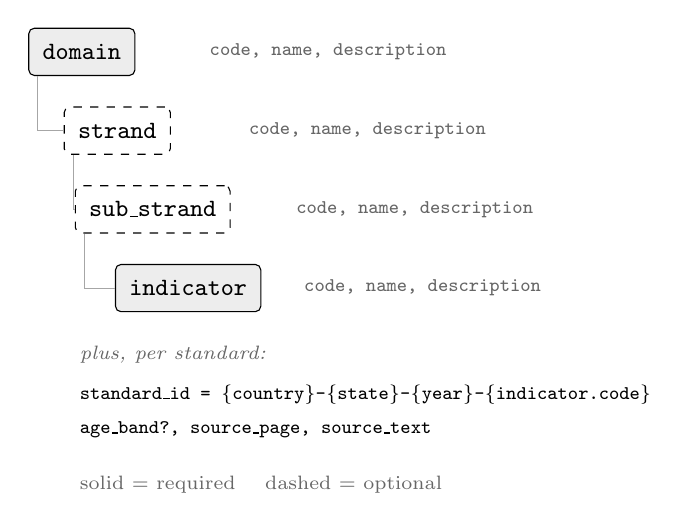
\begin{tikzpicture}[
  font=\small,
  lvl/.style={draw, rounded corners=2pt, minimum height=6mm, inner xsep=5pt, align=left},
  req/.style={lvl, fill=black!7},
  opt/.style={lvl, dashed, fill=white},
  ann/.style={font=\scriptsize\ttfamily, anchor=west, text=black!60},
  link/.style={-, gray!70}
]
\node[req] (d)  at (0,0)      {\texttt{domain}};
\node[opt] (s)  at (0.45,-1)  {\texttt{strand}};
\node[opt] (ss) at (0.90,-2)  {\texttt{sub\_strand}};
\node[req] (i)  at (1.35,-3)  {\texttt{indicator}};

\draw[link] (d.south west) ++(0.12,0) |- (s.west);
\draw[link] (s.south west) ++(0.12,0) |- (ss.west);
\draw[link] (ss.south west) ++(0.12,0) |- (i.west);

\node[ann] at (1.5,0)    {code, name, description};
\node[ann] at (2.0,-1)   {code, name, description};
\node[ann] at (2.6,-2)   {code, name, description};
\node[ann] at (2.7,-3)   {code, name, description};

\node[font=\scriptsize, anchor=west, text=black!60] at (-0.15,-3.85)
  {\textit{plus, per standard:}};
\node[font=\scriptsize\ttfamily, anchor=west] at (-0.15,-4.35)
  {standard\_id = \{country\}-\{state\}-\{year\}-\{indicator.code\}};
\node[font=\scriptsize\ttfamily, anchor=west] at (-0.15,-4.8)
  {age\_band?, source\_page, source\_text};

\node[font=\scriptsize, anchor=west, text=black!60] at (-0.15,-5.5)
  {solid = required \quad dashed = optional};
\end{tikzpicture}
\caption{The canonical schema. Four hierarchy levels, of which
\texttt{strand} and \texttt{sub\_strand} are optional --- Colorado publishes no
sub-strand tier and Texas realizes almost none, so requiring every level would
force the pipeline to invent structure. Each level carries a code, a name and an
optional description. A stored record is one indicator together with its fully
resolved ancestry, not a node in a tree, which is why the identifier embeds the
indicator's already-qualified code and carries any disambiguator itself
(\S\ref{sec:schema}). Every record also retains the source page and the verbatim
text it was extracted from, so any row can be checked against the document that
produced it.}
\label{fig:schema}
\end{figure}


\section{Representative Golden Examples}
\label{sec:appendix-goldens}

% AUTO-GENERATED by paper/analysis/make_goldens_appendix.py -- do not hand-edit.
% Every field is copied from the annotation on disk, so the appendix cannot drift
% from what was actually graded. Regenerate with:
%   python paper/analysis/make_goldens_appendix.py

Both suites are graded against independently annotated golden sets with different shapes: the detector golden is a flat list of elements, the parser golden a nested record per standard. The examples below were each chosen to show one convention the body of the paper turns on. Free-text descriptions are elided for length; codes, levels and identifiers are reproduced in full.

\paragraph{KY \textnormal{---} a \texttt{<Label> <id>} heading, where the label-and-id \emph{is} the code}
\noindent\scriptsize\begin{tabular}{@{}p{0.22\linewidth}p{0.72\linewidth}@{}}
\toprule
\texttt{level} & \texttt{sub\_\allowbreak{}strand} \\
\texttt{code} & \texttt{Benchmark 1.\allowbreak{}1} \\
\texttt{title} & Maintains focus and sustains attention. \\
\texttt{description} & \textit{null} \\
\texttt{source\_page} & 2 \\
\bottomrule
\end{tabular}

\noindent{\scriptsize\raggedright Golden entry \texttt{KY-SUB-01}, \texttt{evaluation/ground\_truth\_detector/KY.json}.\par}

\paragraph{KY \textnormal{---} the same element after parsing, its label form resolved to a domain-qualified code}
\noindent\scriptsize\begin{tabular}{@{}p{0.26\linewidth}p{0.68\linewidth}@{}}
\toprule
\texttt{standard\_id} & \texttt{US-\allowbreak{}KY-\allowbreak{}2021-\allowbreak{}AL.\allowbreak{}1.\allowbreak{}1.\allowbreak{}EASPT} \\
\texttt{domain.code} & \texttt{AL} \\
\texttt{domain.name} & Approaches to Learning \\
\texttt{strand.code} & \texttt{AL.\allowbreak{}1} \\
\texttt{strand.name} & Sustains attention and persists with challenging activities and experiences. \\
\texttt{sub\_strand.code} & \texttt{AL.\allowbreak{}1.\allowbreak{}1} \\
\texttt{sub\_strand.name} & Maintains focus and sustains attention. \\
\texttt{indicator.code} & \texttt{AL.\allowbreak{}1.\allowbreak{}1.\allowbreak{}EASPT} \\
\texttt{indicator.name} & Engages in an activity for a sustained period of time. \\
\texttt{age\_band} & 36-60 \\
\bottomrule
\end{tabular}

\noindent{\scriptsize\raggedright Golden entry \texttt{KY-STD-01}, \texttt{evaluation/ground\_truth\_parser/KY.json}. Descriptions elided.\par}

\paragraph{NV \textnormal{---} a printed namespace that skips a level: the sub-strand code does \emph{not} extend the strand's}
\noindent\scriptsize\begin{tabular}{@{}p{0.26\linewidth}p{0.68\linewidth}@{}}
\toprule
\texttt{standard\_id} & \texttt{US-\allowbreak{}NV-\allowbreak{}2023-\allowbreak{}SS.\allowbreak{}ID.\allowbreak{}PK1} \\
\texttt{domain.code} & \texttt{SS} \\
\texttt{domain.name} & Social Studies \\
\texttt{strand.code} & \texttt{SS.\allowbreak{}1} \\
\texttt{strand.name} & Demonstrate a basic awareness of self as an individual, within the context of a group and community. \\
\texttt{sub\_strand.code} & \texttt{SS.\allowbreak{}ID} \\
\texttt{sub\_strand.name} & Individual Development and Cultural Identity \\
\texttt{indicator.code} & \texttt{SS.\allowbreak{}ID.\allowbreak{}PK1} \\
\texttt{indicator.name} & Identify and describe characteristics of self that are unique from others. \\
\texttt{age\_band} & 36-60 \\
\bottomrule
\end{tabular}

\noindent{\scriptsize\raggedright Golden entry \texttt{NV-STD-01}, \texttt{evaluation/ground\_truth\_parser/NV.json}. Descriptions elided.\par}

\paragraph{CO \textnormal{---} a three-level document --- \texttt{sub\_strand} is absent by design, not missing}
\noindent\scriptsize\begin{tabular}{@{}p{0.26\linewidth}p{0.68\linewidth}@{}}
\toprule
\texttt{standard\_id} & \texttt{US-\allowbreak{}CO-\allowbreak{}2020-\allowbreak{}PDH.\allowbreak{}1.\allowbreak{}1} \\
\texttt{domain.code} & \texttt{PDH} \\
\texttt{domain.name} & Physical Development \& Health \\
\texttt{strand.code} & \texttt{PDH.\allowbreak{}1} \\
\texttt{strand.name} & Health, Safety and Nutrition \\
\texttt{sub\_strand} & \textit{absent --- this document has no such level} \\
\texttt{indicator.code} & \texttt{PDH.\allowbreak{}1.\allowbreak{}1} \\
\texttt{indicator.name} & Possess good overall health, including oral, visual, and auditory health, and be free from communicable or pre [...] \\
\texttt{age\_band} & 36-60 \\
\bottomrule
\end{tabular}

\noindent{\scriptsize\raggedright Golden entry \texttt{CO-IND-01}, \texttt{evaluation/ground\_truth\_parser/CO.json}. Descriptions elided.\par}

\paragraph{CA \textnormal{---} a side-by-side column variant, disambiguated inside the indicator code}
\noindent\scriptsize\begin{tabular}{@{}p{0.26\linewidth}p{0.68\linewidth}@{}}
\toprule
\texttt{standard\_id} & \texttt{US-\allowbreak{}CA-\allowbreak{}2021-\allowbreak{}AL.\allowbreak{}1.\allowbreak{}0.\allowbreak{}INIT.\allowbreak{}1.\allowbreak{}2.\allowbreak{}36-\allowbreak{}54} \\
\texttt{domain.code} & \texttt{AL} \\
\texttt{domain.name} & Approaches to Learning \\
\texttt{strand.code} & \texttt{AL.\allowbreak{}1.\allowbreak{}0} \\
\texttt{strand.name} & Motivation to Learn \\
\texttt{sub\_strand.code} & \texttt{AL.\allowbreak{}1.\allowbreak{}0.\allowbreak{}INIT} \\
\texttt{sub\_strand.name} & Initiative \\
\texttt{indicator.code} & \texttt{AL.\allowbreak{}1.\allowbreak{}0.\allowbreak{}INIT.\allowbreak{}1.\allowbreak{}2.\allowbreak{}36-\allowbreak{}54} \\
\texttt{indicator.name} & Initiative \\
\texttt{age\_band} & 36-54 \\
\bottomrule
\end{tabular}

\noindent{\scriptsize\raggedright Golden entry \texttt{CA-IND-01-EARLY}, \texttt{evaluation/ground\_truth\_parser/CA.json}. Descriptions elided.\par}


\section{Confidence Score Distribution}
\label{sec:appendix-confidence}

Table~\ref{tab:confidence-distribution} gives the detector's confidence
distribution by state and by hierarchy level, read by
\S\ref{sec:experiments-confidence}. It is in the appendix because the score
gates nothing in the pipeline and the section's conclusion, that the
distribution is too degenerate to threshold on, is carried by the prose.

% AUTO-GENERATED by paper/analysis/generate_tables.py -- do not hand-edit.
% Source: paper/results/task8_20260904/confidence_distribution.json
% Regenerate with: python paper/analysis/generate_tables.py
% Corpus tier (guardrail 1): every row is the _only_subset tier, never full-document.
\begin{table}
  \centering
  \small
  \begin{tabular}{lrrr}
    \hline
    & \textbf{n} & \textbf{Range} & $\mathbf{\geq 0.95}$ \\
    \hline
    \multicolumn{4}{l}{\emph{By hierarchy level}} \\
    domain & 16 & 0.95--0.97 & 16/16 \\
    strand & 51 & 0.92--0.97 & 48/51 \\
    sub-strand & 49 & 0.92--0.97 & 47/49 \\
    indicator & 263 & 0.90--0.97 & 246/263 \\
    \hline
    \multicolumn{4}{l}{\emph{By human false-positive audit verdict}} \\
    matched a golden & 135 & 0.92--0.97 & 117/135 \\
    real, unannotated & 117 & 0.92--0.97 & 115/117 \\
    real, split title & 39 & 0.95--0.96 & 39/39 \\
    real, reprinted & 5 & 0.95--0.95 & 5/5 \\
    \textbf{invented} & 1 & 0.90--0.90 & 0/1 \\
    \hline
    All & 379 & 0.90--0.97 & 357/379 \\
    \hline
  \end{tabular}
  \caption{Detector self-reported confidence, re-measured over the 379 elements of the recorded run. The prompt asks for $\geq 0.95$ when the depth map clearly applies, $0.80$--$0.94$ when the chunk is ambiguous, and $<0.70$ when guessing; the score in fact takes 5 distinct values in $[0.90, 0.97]$ and uses the bottom band never. \textbf{Nothing in the pipeline thresholds this score} (\S\ref{sec:experiments-confidence}). \emph{\_only\_subset} tier. Source: \texttt{task8\_20260904}.}
  \label{tab:confidence-distribution}
\end{table}

% Moved out of the body 2026-09-07: Table 6 was the least load-bearing table in
% \S6, and the confidence finding is negative; the table's job is to let a
% reader check the degeneracy claim, not to carry it.

\section{Corpus}
\label{sec:appendix-corpus}

Table~\ref{tab:corpus-appendix} identifies every source document by publisher,
year and page count at each tier, and Table~\ref{tab:corpus-pages} gives the
pages of each published PDF that the \texttt{\_trimmed} and
\texttt{\_only\_subset} tiers retain, in the published document's own page
numbering, so that the trimming can be reproduced exactly from the issuing
agency's copy (\S\ref{sec:corpus}).

% AUTO-GENERATED by paper/analysis/generate_tables.py -- do not hand-edit.
% Source: standards/standards_tracking.md, paper/results/corpus_tiers.json
% Regenerate with: python paper/analysis/generate_tables.py
% Corpus tier (guardrail 1): every row is the _only_subset tier, never full-document.
\begin{table*}[t]
\centering
\small
\begin{tabular}{llrlrrr}
\toprule
\textbf{State} & \textbf{Role} & \textbf{Year} & \textbf{Publisher} & \textbf{Full} & \textbf{Trim.} & \textbf{Subset} \\
\midrule
CA & dev & 2021 & CA Dept.\ of Education & 68 & -- & 13 \\
AZ & dev & 2018 & AZ Dept.\ of Education & 217 & 65 & 15 \\
TX & dev & 2022 & TX Education Agency & 87 & 71 & 9 \\
CO & dev & 2020 & CO Dept.\ of Early Childhood & 41 & 41 & 10 \\
NV & held-out & 2023 & NV Dept.\ of Education & 98 & 71 & 15 \\
KY & held-out & 2021 & Governor's Office of Early Childhood & 120 & 52 & 8 \\
\midrule
\multicolumn{7}{l}{\emph{Collected, not used --- excluded from every measurement in this paper}} \\
NV & -- & 2025 & NV Dept.\ of Education & 36 & -- & -- \\
\bottomrule
\end{tabular}
\caption{Corpus provenance. \emph{Full} is the published PDF; \emph{Trim.}\ removes non-standards matter while retaining every standard; \emph{Subset} is the one-to-two-domain excerpt all quality measurements use, and is a genuine reduction in coverage. Colorado's \emph{Full} is its 41-page Ages~3--5 publication (\S\ref{sec:corpus}). These are third-party state-agency documents, identified here rather than redistributed (\S\ref{sec:artifacts-statement}). Nevada's 2025 publication covers the \textbf{social-emotional domain only}; it is listed because Nevada is the only state with two published documents, and every Nevada number in this paper refers to the 2023 one. Page counts verified with PyMuPDF. Source: \texttt{standards\_tracking.md}, \texttt{corpus\_tiers.json}.}
\label{tab:corpus-appendix}
\end{table*}

% AUTO-GENERATED by paper/analysis/generate_tables.py -- do not hand-edit.
% Source: paper/results/corpus_page_ranges.json
% Regenerate with: python paper/analysis/generate_tables.py
% Corpus tier (guardrail 1): this table DESCRIBES the tiers themselves and carries no quality number.
\begin{table*}[t]
\centering
\small
\begin{tabular}{llrp{0.40\textwidth}p{0.22\textwidth}}
\toprule
\textbf{State} & \textbf{Tier} & \textbf{pp} & \textbf{Retained, by PDF page index} & \textbf{Same pages, as printed} \\
\midrule
AZ & \texttt{\_trimmed} & 65 & 2, 21, 23--28, 41, 43--50, 66, 70--82, 107, 110--120, 139, 142--145, 156, 158--162, 179, 181--185, 198, 201--204 (of 217) & 18, 20--25, 38, 40--47, 63, 67--79, 104, 107--117, 136, 139--142, 153, 155--159, 176, 178--182, 195, 198--201 \\
AZ & \texttt{\_only\_subset} & 15 & 2, 21, 23, 66, 70--78, 81--82 (of 217) & 18, 20, 63, 67--75, 78--79 \\
CA & \texttt{\_only\_subset} & 13 & 1--5, 11--13, 18--22 (of 68) & \emph{not recovered} \\
CO & \texttt{\_trimmed} & 41 & 1--41 (of 41) & \emph{not recovered} \\
CO & \texttt{\_only\_subset} & 10 & 1, 3--9, 11--12 (of 41) & \emph{not recovered} \\
TX & \texttt{\_trimmed} & 71 & 1, 9--65, 69--81 (of 87) & \emph{not recovered} \\
TX & \texttt{\_only\_subset} & 9 & 1, 9--13, 59--61 (of 87) & \emph{not recovered} \\
NV & \texttt{\_trimmed} & 71 & 1, 3, 16--84 (of 98) & \emph{not recovered} \\
NV & \texttt{\_only\_subset} & 15 & 1, 3, 23--26, 54--57, 61--65 (of 98) & \emph{not recovered} \\
KY & \texttt{\_trimmed} & 52 & 1, 52--102 (of 120) & 39--89 \\
KY & \texttt{\_only\_subset} & 8 & 1, 52--55, 65, 71--72 (of 120) & 39--42, 52, 58--59 \\
\bottomrule
\end{tabular}
\caption{Pages retained at each corpus tier, so the hand trimming can be reproduced from the issuing agency's copy. \textbf{Two numberings are given and they are not interchangeable}: the PDF page index counts pages in the file, while the printed number is what appears on the page, and they differ by each document's unnumbered front matter (Kentucky's PDF page 52 is printed page 39). Navigate a file by the first and a paper copy by the second. Ranges were recovered by matching each tier page's text back to the published PDF; no annotation or model call is involved. The printed column is populated only where page-number extraction is reliable across the tier, and left blank rather than guessed otherwise. Every tier page matched a published page. California has no \texttt{\_trimmed} tier and Colorado's is the whole document. Source: \texttt{corpus\_page\_ranges.json}.}
\label{tab:corpus-pages}
\end{table*}


% system_architecture.tex — Task 10 stub. Outline recovered verbatim from
% the original plan file fragment (see ../OUTLINE_NOTES.md). Draft at Task 12.
%
% Serverless stages ingestion -> extraction -> detection -> parsing ->
% validation -> persistence; prepare -> Step Functions Map -> merge
% batching; S3-as-bus intermediates. Note the batched production path
% differs from the direct path the evals use — say so (see
% tasking/arxiv_paper.md's batched-vs-direct background note).

\section{System Architecture}
\label{sec:system-architecture}

\begin{figure*}
  \centering
  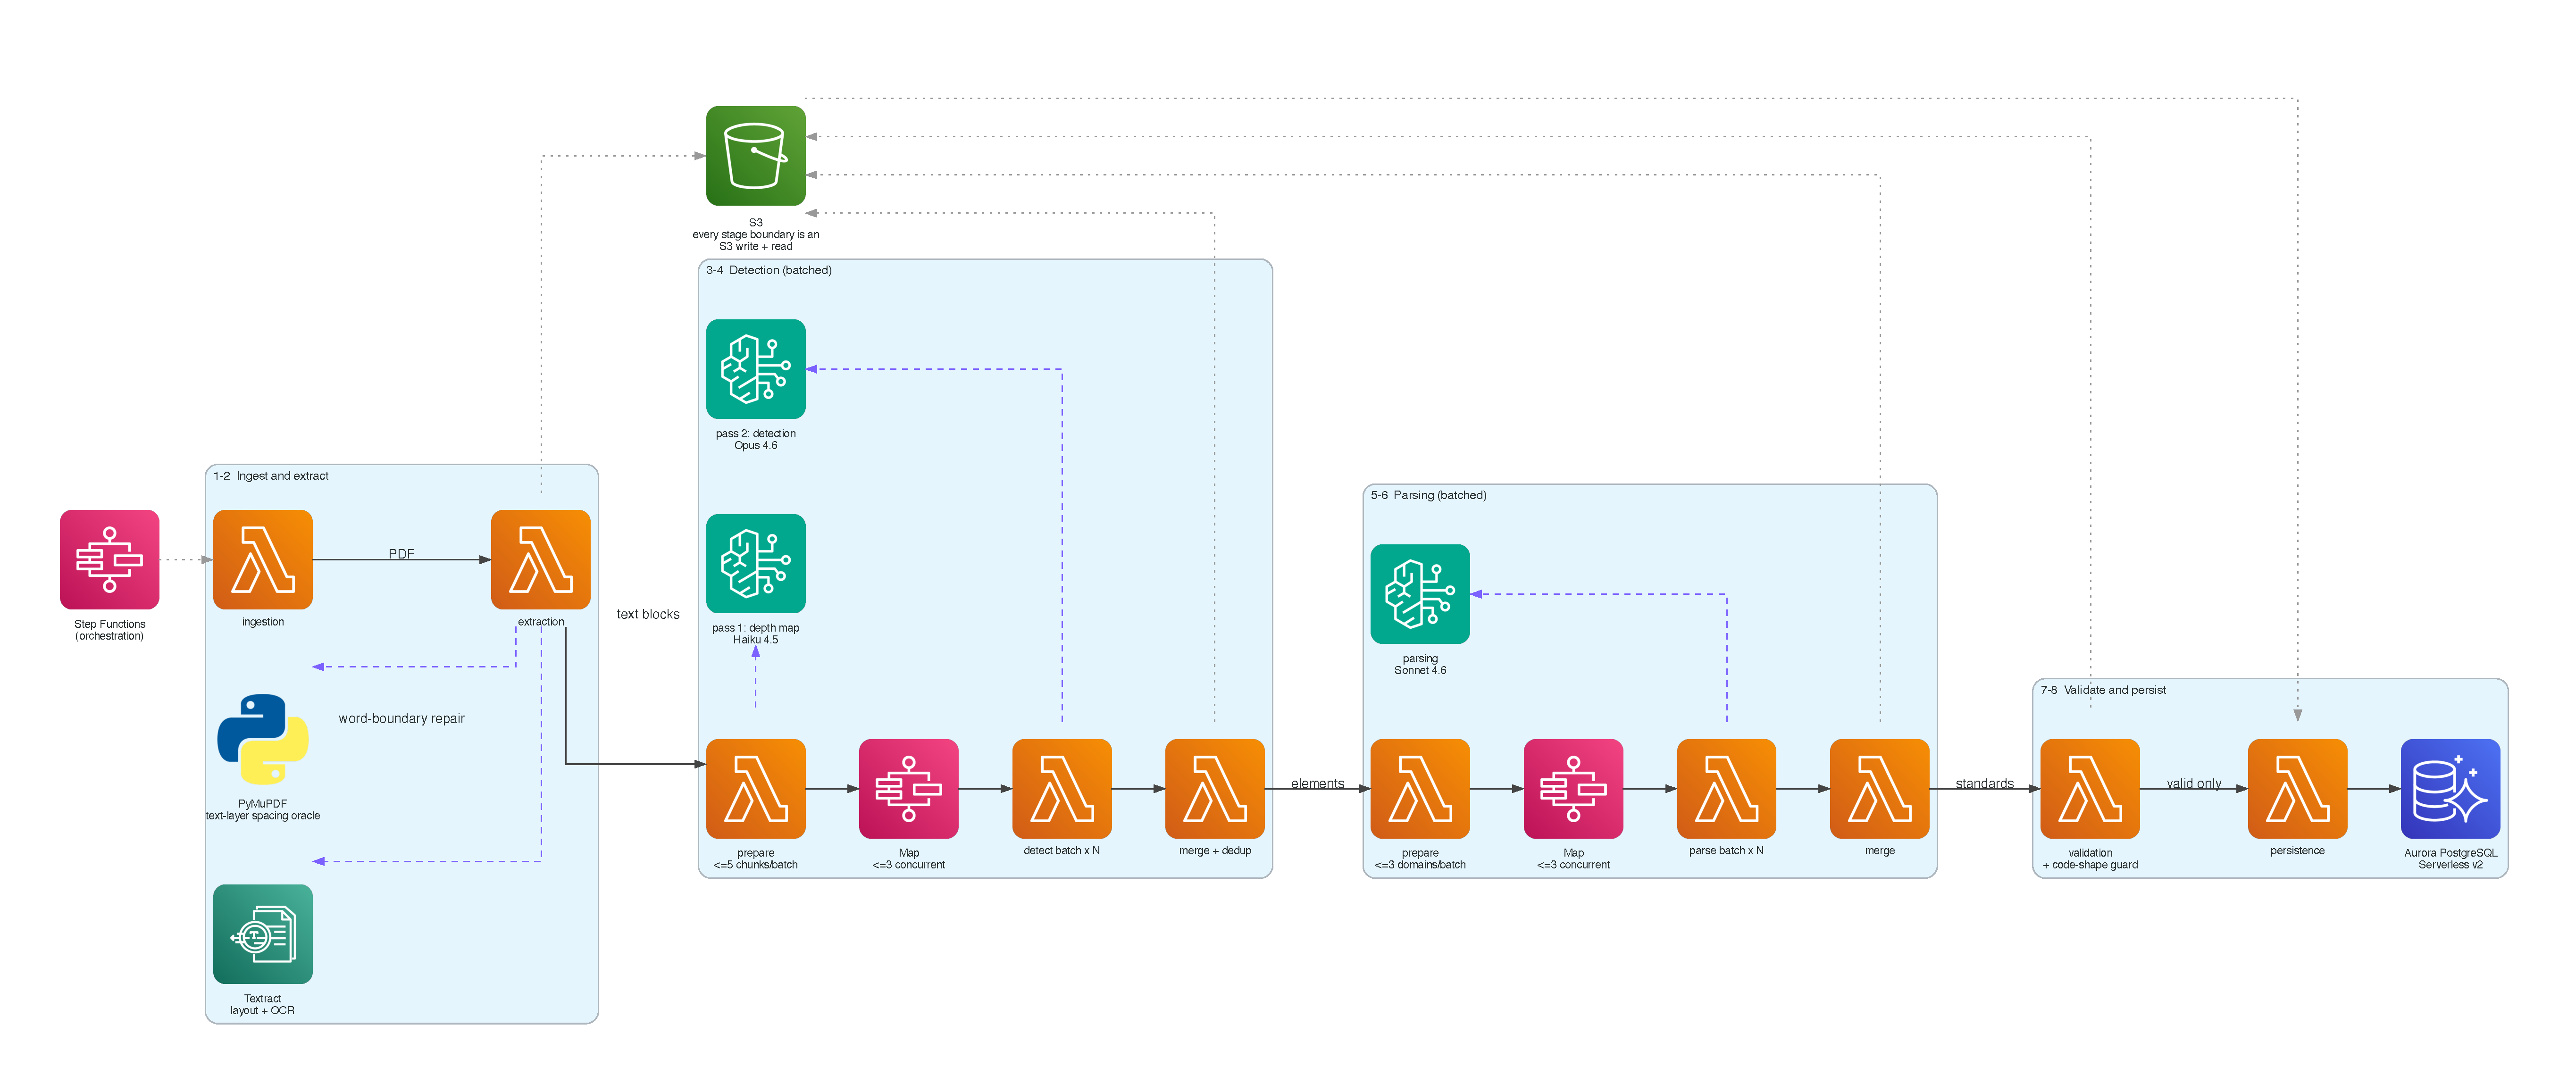
\includegraphics[width=\textwidth]{figures/fig_architecture.pdf}
  \caption{Pipeline architecture. Solid arrows carry data, dashed arrows are
  model calls, and dotted arrows mark JSON exchanged through S3. Regenerate with
  \texttt{python paper/analysis/make\_architecture\_figure.py}.}
  \label{fig:architecture}
\end{figure*}

Figure~\ref{fig:architecture} shows the deployed system. Documents flow through
the six pipeline stages of \S\ref{sec:pipeline-overview}, numbered 1--8 in the
figure because the two batched stages each occupy two positions --- prepare,
then map and merge --- and are realized as ten Lambda handlers in all. Stages
communicate by writing JSON to S3 rather than by passing payloads directly, so
each stage's input and output can be inspected in isolation when a run is
debugged.

Detection and parsing are batched through a prepare $\rightarrow$ Step Functions
\texttt{Map} $\rightarrow$ merge pattern, with at most three concurrent workers,
so that a long document does not exhaust the Lambda timeout. Detection batches
by text-block chunk and parsing by domain, which keeps related elements in the
same call. Detection is itself two-pass: the depth-map pass infers the
document's nesting hierarchy before any element is classified against it.

\textbf{The evaluation suites exercise the direct path rather than this batched
one, and the two are known to diverge} (\S\ref{sec:discussion-limitations}).
Every quality number in this paper is therefore a measurement of the direct
path, and Table~\ref{tab:scale} is the only evidence here that the batched path
behaves as intended.

% Standards Explorer screenshot — supplied by Emily 2026-09-04 as
% figures/colorado_els.png, replacing an earlier Arizona capture whose document
% title read "SUBSET - Arizona Early Learning Standards". That title would have
% invited the reader to conclude the PRODUCT only ever holds subsets, which is a
% stronger and false claim than the subset-tier EVALUATION the paper discloses.
% This capture is Colorado at the _trimmed tier: the complete Ages 3-5 document.
% Checked before inclusion: no account IDs, ARNs, internal URLs or email
% addresses are visible.
Figure~\ref{fig:explorer} shows the end of that pipeline as a user meets it:
extracted standards resolved into the canonical schema and served through the
Standards Explorer, where the per-element verification workflow of
\S\ref{sec:method-confidence} is carried out.

\begin{figure*}[t]
  \centering
  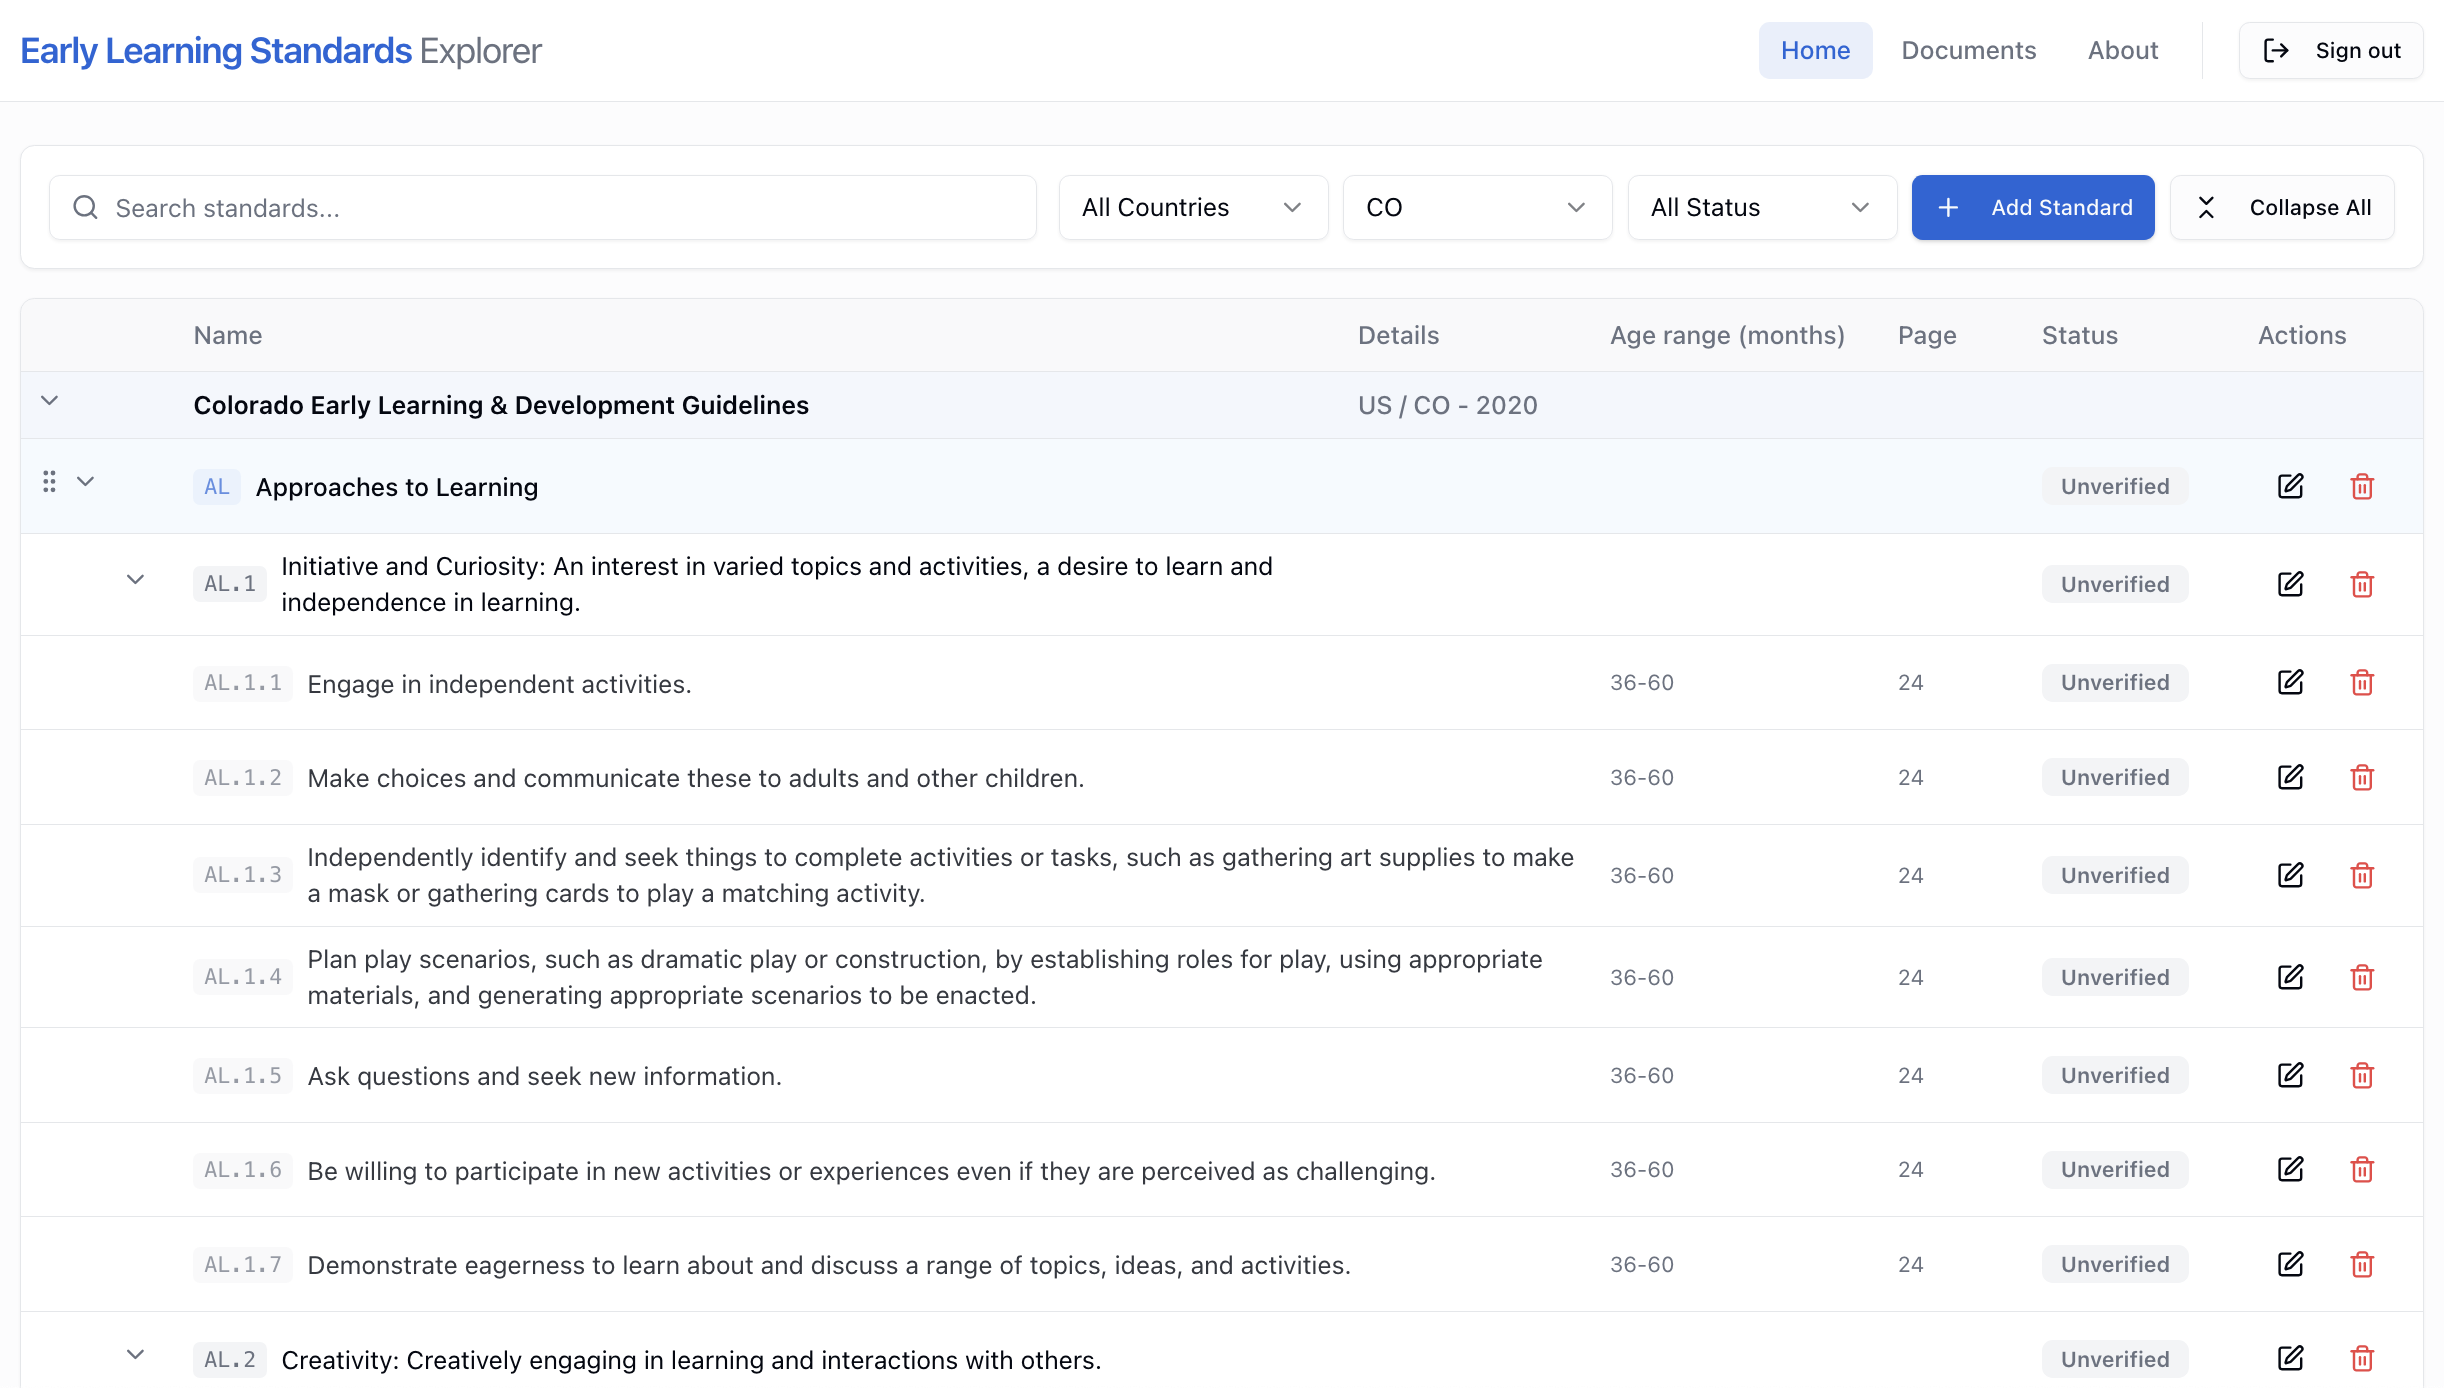
\includegraphics[width=\textwidth]{figures/colorado_els.png}
  \caption{The Standards Explorer, showing extracted Colorado standards resolved
  into the canonical schema of \S\ref{sec:schema}: domain \texttt{AL}, strand
  \texttt{AL.1}, and the indicators beneath it, each row carrying its age range
  and source page. The \emph{Status} column is the per-element human
  verification state of \S\ref{sec:method-confidence}, which is
  \textbf{independent of the model's confidence score}.}
  \label{fig:explorer}
\end{figure*}

% Moved out of the body 2026-09-07 (REVIEW_assessment.md §2): the architecture
% figure and the Explorer screenshot are deployment detail, and the two claims
% the body needs from them (the batching pattern and the direct-vs-batched
% divergence) are stated in \S\ref{sec:method-deployment}.

\end{document}
